\documentclass[12pt,a4paper,oneside]{report}

% ==============================================================================
% PRÉAMBULE (Packages essentiels)
% ==============================================================================
\usepackage[utf8]{inputenc}
\usepackage[T1]{fontenc}
\usepackage[french]{babel}
\usepackage[normalem]{ulem}
\usepackage{graphicx} % Pour les images et l'organigramme PDF
\usepackage{float}
\usepackage{amsmath,amssymb}
\usepackage{geometry}
\usepackage{titlesec}
\usepackage{indentfirst}
\usepackage{enumitem}
\usepackage{tocloft}
\usepackage{needspace}
\usepackage{etoc}

% Positionne et centre le titre du sommaire.
\setlength{\cftbeforetoctitleskip}{0pt}
\setlength{\cftaftertoctitleskip}{0.5em}
\setlength{\cftbeforechapskip}{0.5cm}
\setlength{\cftbeforesecskip}{0.9em}
\setlength{\cftbeforesubsecskip}{0.3em}
\setlength{\cftbeforeparaskip}{0.2em}
\renewcommand{\cfttoctitlefont}{\centering\Huge\bfseries}
\renewcommand{\cftaftertoctitle}{\par}
\renewcommand{\cftchapfont}{\large\bfseries}
\renewcommand{\cftchappagefont}{\large\bfseries}
\renewcommand{\cftsecfont}{\ttfamily}

\geometry{top=2.5cm, bottom=2.5cm, left=2.5cm, right=2.5cm}

\newcommand{\textsb}[1]{{\fontseries{sb}\selectfont #1}}
\newcommand{\bulle}{\textbullet}

\makeatletter
\newcommand{\printannextoc}{%
    \begingroup
    \section*{Sommaire des annexes}
    \@starttoc{annextoc}
    \endgroup
}

\newcommand{\annexchapter}[1]{%
    \refstepcounter{chapter}%
    \chapter*{\thechapter\quad #1}%
    \addcontentsline{annextoc}{chapter}{\protect\numberline{\thechapter}#1}%
}

\newcommand{\annexsection}[1]{%
    \refstepcounter{section}%
    \section*{\thesection\quad #1}%
    \addcontentsline{annextoc}{section}{\protect\numberline{\thesection}#1}%
}

\newcommand{\annexsubsection}[1]{%
    \refstepcounter{subsection}%
    \subsection*{\thesubsection\quad #1}%
    \addcontentsline{annextoc}{subsection}{\protect\numberline{\thesubsection}#1}%
}

\newcommand{\annexsubsubsection}[1]{%
    \refstepcounter{subsubsection}%
    \subsubsection*{\thesubsubsection\quad #1}%
    \addcontentsline{annextoc}{subsubsection}{\protect\numberline{\thesubsubsection}#1}%
}
\makeatother

\usepackage{tikz}
\usetikzlibrary{shapes,arrows,positioning,calc}
\usepackage{hyperref} % Pour les liens cliquables
\hypersetup{colorlinks=true, linkcolor=black, urlcolor=blue}

\titleformat{\chapter}[display]
    {\normalfont\Huge\bfseries}
    {\chaptertitlename\ \thechapter}
    {20pt}
    {}
\titlespacing*{\chapter}{0pt}{0pt}{1em}
\titleformat{\section}
    {\normalfont\LARGE\bfseries}
    {\thesection}
    {1em}
    {}
\titleformat{\subsection}
    {\normalfont\Large\bfseries}
    {\thesubsection}
    {1em}
    {}
\titleformat{\subsubsection}
    {\normalfont\large\bfseries}
    {\thesubsubsection}
    {1em}
    {}

\begin{document}

% ==============================================================================
% PAGE DE GARDE RESTRUCTURÉE (MODÈLE OFFICIEL)
% ==============================================================================
\begin{titlepage}
    \centering
    
    % Logos alignés en haut
    \noindent
    \begin{minipage}[c]{0.125\textwidth}
        
\includegraphics[width=\textwidth]{img_garde/logo_uca.png}
    \end{minipage}
    \hfill
    \begin{minipage}[c]{0.4\textwidth}
        \centering
        
\includegraphics[width=\textwidth]{img_garde/logo_eupi.png}
    \end{minipage}
    \hfill
    \begin{minipage}[c]{0.125\textwidth}
        \flushright
        
\includegraphics[width=\textwidth]{img_garde/logo_institut.png}
    \end{minipage}
    
    \vspace{1.5cm}
    
    % 1. Bloc Institutionnel (Haut)
    {\large \textbf{UNIVERSITÉ CLERMONT AUVERGNE} \\ Clermont-Ferrand \par}
    \vspace{0.2cm}
    {---- \par}
    \vspace{0.2cm}
    {\large École Universitaire de Physique et d'Ingénierie \par}
    \vspace{0.2cm}
    {---- \par}
    
    \vspace{2cm}
    
    % 2. Bloc Diplôme & Spécialité (Milieu)
    {\LARGE \textbf{MÉMOIRE DE STAGE} \par}
    \vspace{0.4cm}
    {\Large 1\textsuperscript{ère} année de Master \par}
    \vspace{0.2cm}
    {---- \par}
    \vspace{0.2cm}
    {\large Spécialité : Automatique et Robotique \par}
    
    \vspace{2cm}
    
    % 3. Bloc Étudiant & Titre
    {\large \textbf{Romaric PRADEAU} \par}
    \vspace{0.8cm}
    {\LARGE \textbf{Calibration de capteurs hétérogènes LiDAR-Caméra \\ par analyse géométrique basée sur l'IA} \par}
    
    \vfill
    
    % 4. Bloc Informations Entreprise & Soutenance (Bas Gauche)
    \begin{flushleft}
        \large
        \textbf{Date de soutenance :} Septembre 2026 \par
        \vspace{0.2cm}
        \textbf{Entreprise :} Institut Pascal (UMR 6602)
    \end{flushleft}
    
\end{titlepage}

% ==============================================================================
% PAGES PRÉLIMINAIRES (Numérotation romaine masquée)
% ==============================================================================
\pagenumbering{roman} 
\thispagestyle{empty} % Supprime le numéro sur la page courante

% ==============================================================================
% REMERCIEMENTS
% ==============================================================================

\begin{center}
    {\Huge\bfseries Remerciements}   
\end{center}
\addcontentsline{toc}{chapter}{Remerciements}
\thispagestyle{empty} % Supprime le numéro "i" en bas des remerciements

\vspace{2cm}

\textit{En préambule à la présentation de mon rapport de stage, je tiens à exprimer tous mes remerciements à toutes les personnes qui ont permis le bon déroulement de celui-ci ainsi que l'expérience que j'ai pu en retirer.}\vspace{2cm}

- \textbf{M. Thierry CHATEAU} et \textbf{M. François MARMOITON}, mes maîtres de stage, pour leur disponibilité constante, leur patience et la pertinence de leur encadrement \\
Leurs conseils avisés, leurs connaissances techniques en robotique ainsi que leur vision scientifique m'ont aidé tout au long de la structuration de ma méthode de calibration.\vspace{0.5cm}

Mes remerciements s'adressent également aux partenaires du projet \textbf{PAVIN} pour leur collaboration et le grand intérêt porté à mes travaux.\vspace{0.5cm}

Je salue chaleureusement l'ensemble des ingénieurs, chercheurs et doctorants de l'équipe pour leur accueil, leur aide précieuse au quotidien — notamment lors de la prise en main de ROS 2 et des phases d'expérimentation sur les plateformes du laboratoire — ainsi que pour la très bonne ambiance de travail.\vspace{1cm}

Enfin, je remercie l'équipe pédagogique de l'\textbf{École Universitaire de Physique et d'Ingénierie (EUPI)} et de l'Université Clermont Auvergne, tout particulièrement les enseignants de la spécialité \textit{Automatique et Robotique}, pour les connaissances théoriques et pratiques qu'ils m'ont transmises et qui m'ont permis de mener à bien ce projet d'intelligence artificielle appliquée à la vision et aux LiDAR.\vspace{1cm}

Je n'oublie pas ma famille et mes amis pour leur soutien inconditionnel et leurs encouragements tout au long de mon parcours universitaire.\vspace{0.5cm}


\newpage

% ==============================================================================
% RÉSUMÉ
% ==============================================================================
\begin{center}
    {\Huge\bfseries Introduction}\par
    \vspace{0.5cm}
    {\Large\bfseries Objectif du stage: Auto-calibration d'un système avec ses différents périphériques hétérogènes}
\end{center}
\addcontentsline{toc}{chapter}{Objectif du stage}
\thispagestyle{empty} % Supprime le numéro en bas du résumé

\bigskip

\hspace*{1cm}Mon stage de Master 1 a été consacré à l'étude de la calibration extrinsèque hétérogène entre capteurs LiDAR et caméras sur une plateforme autonome.\\

\hspace*{1cm}Mon travail s'inscrivait dans le cadre de la perception multi-capteurs et visait à améliorer la robustesse des systèmes de navigation intelligents en environnement réel, notamment pour les véhicules autonomes et les robots mobiles. \\
\hspace*{1cm}Le contexte scientifique du projet s'appuyait sur le constat que les données issues de capteurs variés sont souvent acquises dans des référentiels différents, avec des cadences, des résolutions et des erreurs de synchronisation distinctes. \\

Cette hétérogénéité compliquait fortement l'estimation précise des poses relatives, alors même que cette étape était déterminante pour la reconstruction 3D, la perception environnementale et la navigation autonome.

\bigskip

Dans ce cadre, l'étude a porté sur le comportement du modèle d'intelligence artificielle \textbf{VGGT} (\textit{Visual Geometry Grounded Transformer}) appliqué à des séquences d'images issues de véhicules autonomes. \\
\hspace*{.3cm}Les principaux verrous identifiés concernaient la qualité et la cohérence géométrique des données alimentant le réseau. Les séquences brutes contenaient :
\begin{itemize}[label=\textbullet]
    \item \textbf{des vues redondantes}
    \item \textbf{des phases stationnaires}
    \item \textbf{des artefacts de synchronisation}
    \item \textbf{des informations peu utiles pour la calibration}
\end{itemize}

\bigskip

Afin de répondre à cette problématique, un pipeline de prétraitement structuré a été mis en œuvre et développé : 
\begin{itemize}[label=\textbullet]
    \item \textbf{Filtrage cinématique}
    \item \textbf{Sélection visuelle intelligente}
    \item \textbf{Génération d'une vérité terrain à partir de données LiDAR et SLAM}
\end{itemize}

\bigskip

Mon travail a aussi porté sur trois axes complémentaires :
    \begin{itemize}[label=\textbullet]
    \item \textbf{La synchronisation temporelle des flux hétérogènes}
    \item \textbf{La sélection d'images non pertinentes}
    \item \textbf{La mise en place d'une stratégie de comparaison avec une référence géométrique}
\end{itemize}

\hspace*{1cm} Les données odométriques du véhicule, les informations GPS, les nuages de points LiDAR et les appariements visuels par \textbf{LoFTR} ont notamment été exploités afin de sélectionner des vues à forte valeur géométrique.\\
Cette approche a permis d'atténuer la charge de calcul du modèle en limitant les redondances et en améliorant la stabilité des estimations de poses.

% Pour la Présentation
%À l'issue de ce stage, le système développé a permis d'évaluer la capacité du modèle à estimer des trajectoires et des relations extrinsèques dans un environnement complexe, en particulier autour d'un rond-point. Les résultats démontrent que la qualité du prétraitement est un élément central du succès d'un réseau de vision géométrique. Le mémoire montre que les performances dépendent autant du modèle que de la manière dont les données sont filtrées, synchronisées et comparées à une référence de terrain. Cette conclusion ouvre des perspectives importantes pour la suite du projet, notamment l'intégration d'une calibration plus robuste, la génération d'images de synthèse à partir du LiDAR et l'optimisation plus fine de l'alimentation des réseaux d'apprentissage profond.

\newpage

% ==============================================================================
% SOMMAIRE ET TABLES
% ==============================================================================
\thispagestyle{empty}
\tableofcontents

\newpage

% ==============================================================================
% CORPS DU RAPPORT : PASSAGE AUX CHIFFRES ARABES (1, 2, 3...)
% ==============================================================================
\pagenumbering{arabic} % Recommence proprement la numérotation à 1 ici !

% ==============================================================================
% PREMIÈRE PARTIE : PRÉSENTATION DE L'ENTREPRISE ET DU SERVICE
% ==============================================================================
\chapter{Présentation de l'entreprise et du service}

\vspace{1cm}

\section{L'entreprise}
Mon stage de Master 1 en Automatique et Robotique s'est déroulé à l'\textbf{Institut Pascal}, unité mixte de recherche située sur le campus des Cézeaux à Aubière.
%L'accueil d'un stagiaire au sein d'une structure de recherche ou d'une entreprise nécessite une compréhension globale de son environnement macroéconomique, institutionnel et structurel. C'est dans ce cadre que cette section présente l'Institut Pascal, l'unité mixte de recherche au sein de laquelle s'est déroulé ce stage de Master 1 en Automatique et Robotique.

\vspace{1cm}

\subsection{Carte d'identité et caractéristiques}
L'Institut Pascal est une Unité Mixte de Recherche (UMR 6602) caractérisée par une forte interdisciplinarité, combinant recherches fondamentales et technologiques ainsi que des formations de haut niveau. Ses principales caractéristiques administratives et institutionnelles sont synthétisées dans le tableau~\ref{tab:carte_identite}.

\vspace{2cm}

\begin{table}[htbp]
    \centering
    \small
    \renewcommand{\arraystretch}{1.6}
    \begin{tabular}{|l|l|}
        \hline
        \textbf{Caractéristique} & \textbf{Détails institutionnels} \\
        \hline
        \textbf{Nom officiel} & Institut Pascal (UMR 6602) \\
        \hline
        \textbf{Statut juridique} & Unité Mixte de Recherche (Établissement public) \\
        \hline
        \textbf{Tutelles principales} & Université Clermont Auvergne (UCA) et CNRS (INSIS principal) \\
        \hline
        \textbf{Tutelles secondaires} & CHU de Clermont-Ferrand, INS2I, INP \\
        \hline
        \textbf{Rattachement ingénieur} & Clermont Auvergne INP (ISIMA, POLYTECH, SIGMA) \\
        \hline
        \textbf{Date de création} & 2012 (puis extensions en 2017 et 2021) \\
        \hline
        \textbf{Effectif global} & Environ 400 personnels (titulaires, doctorants et contractuels) \\
        \hline
        \textbf{Adresse principale} & Campus des Cézeaux, 4 Av. Blaise Pascal, 63178 Aubière Cedex \\
        \hline
        \textbf{Téléphone} & +33 (0)4 73 40 72 50 \\
        \hline
    \end{tabular}
    \caption{Carte d'identité institutionnelle de l'Institut Pascal}
    \label{tab:carte_identite}
\end{table}

\newpage

\subsection{Historique de l'entreprise}
L'Institut Pascal est une structure moderne née d'une volonté politique et académique de structurer et de fédérer les forces de recherche en ingénierie sur le site clermontois. Son évolution s'articule autour de trois jalons chronologiques essentiels :
\begin{itemize}
    \item \textbf{2012 : Création initiale.} Fusion fondatrice visant à regrouper plusieurs laboratoires pionniers du site clermontois afin de créer une synergie interdisciplinaire forte.
    \item \textbf{2017 : Deuxième phase d'extension.} Intégration de nouvelles thématiques de recherche pour couvrir de manière plus exhaustive les disciplines des Sciences de l'Ingénierie et des Systèmes.
    \item \textbf{2021 : Consolidation finale.} Intégration de 7 laboratoires au total, consolidant les thématiques de recherche phares : Génie des Procédés, Mécanique, Robotique, Physique des Sciences de l'Information, et Santé.
\end{itemize}

\subsection{Implantation géographique}
Bien que la direction générale et le cœur historique de l'Institut Pascal soient basés à Aubière, la structure présente une organisation stratégique multi-sites afin de collaborer étroitement avec les centres hospitaliers et les antennes universitaires régionales.\\
Les forces vives sont réparties de la manière suivante :
\begin{enumerate}
    \item \textbf{Site principal (Campus des Cézeaux) :} Accueille la direction, l'administration centrale ainsi que les équipes adossées à l'EUPI, Polytech Clermont et SIGMA Clermont.
    \item \textbf{Site Hospitalier (CHU de Clermont-Ferrand) :} Situé au sein des hôpitaux Gabriel Montpied et d'Estaing pour les recherches en technologies de la santé (Thérapies Guidées par l'Image).
    \item \textbf{Sites territoriaux :} Les antennes délocalisées de Montluçon (IUT d'Allier) et du Puy-en-Velay (IUT de Clermont).
\end{enumerate}

\begin{figure}[htbp]
    \centering
    \makebox[\textwidth][c]{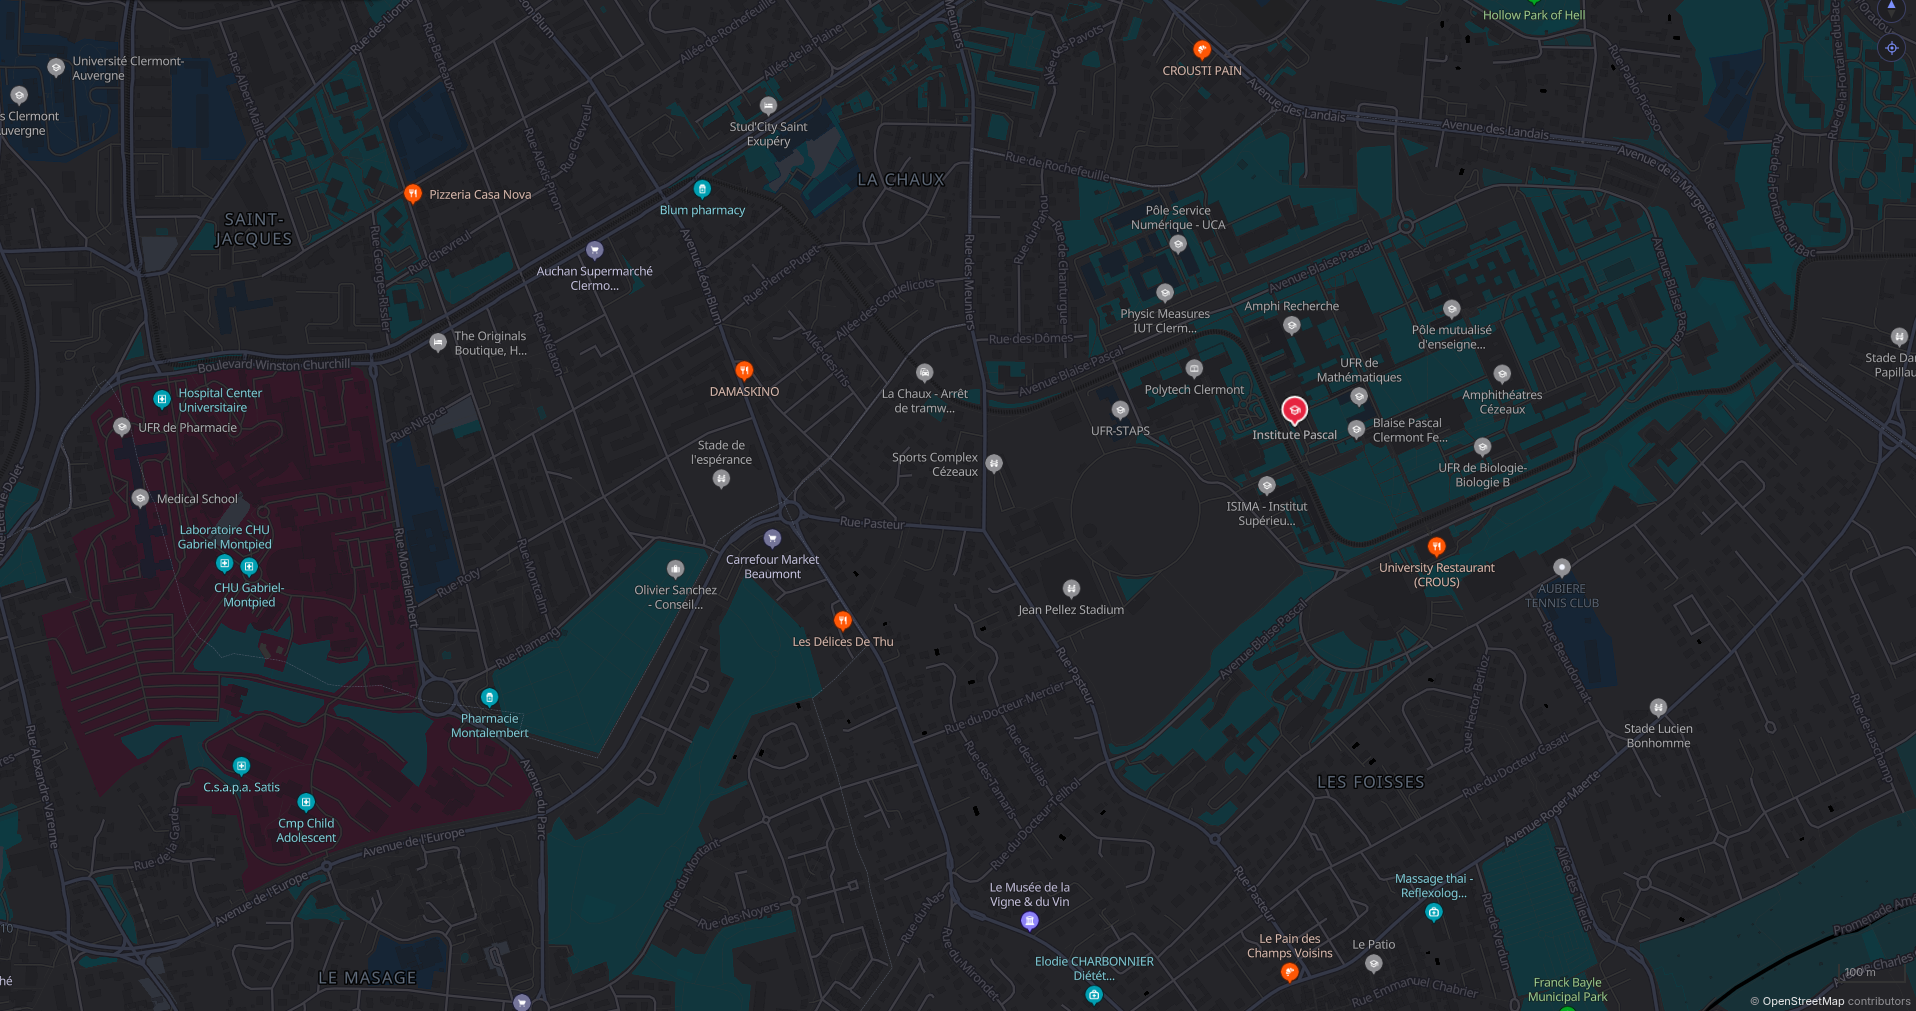
\includegraphics[width=0.8\textwidth]{img/map_institut.png}}
    \caption{Implantation du site principal de l'Institut Pascal sur le campus des Cézeaux}
    \label{fig:implantation}
\end{figure}

\vspace*{\fill}

L'implantation sur le Campus des Cézeaux (illustrée par la figure~\ref{fig:implantation}) offre une proximité immédiate avec les infrastructures de l'École Universitaire de Physique et d'Ingénierie (EUPI), facilitant le continuum entre formations et recherches d'excellence.

\bigskip
\bigskip

\begin{figure}[H]
    \centering
    \makebox[\textwidth][c]{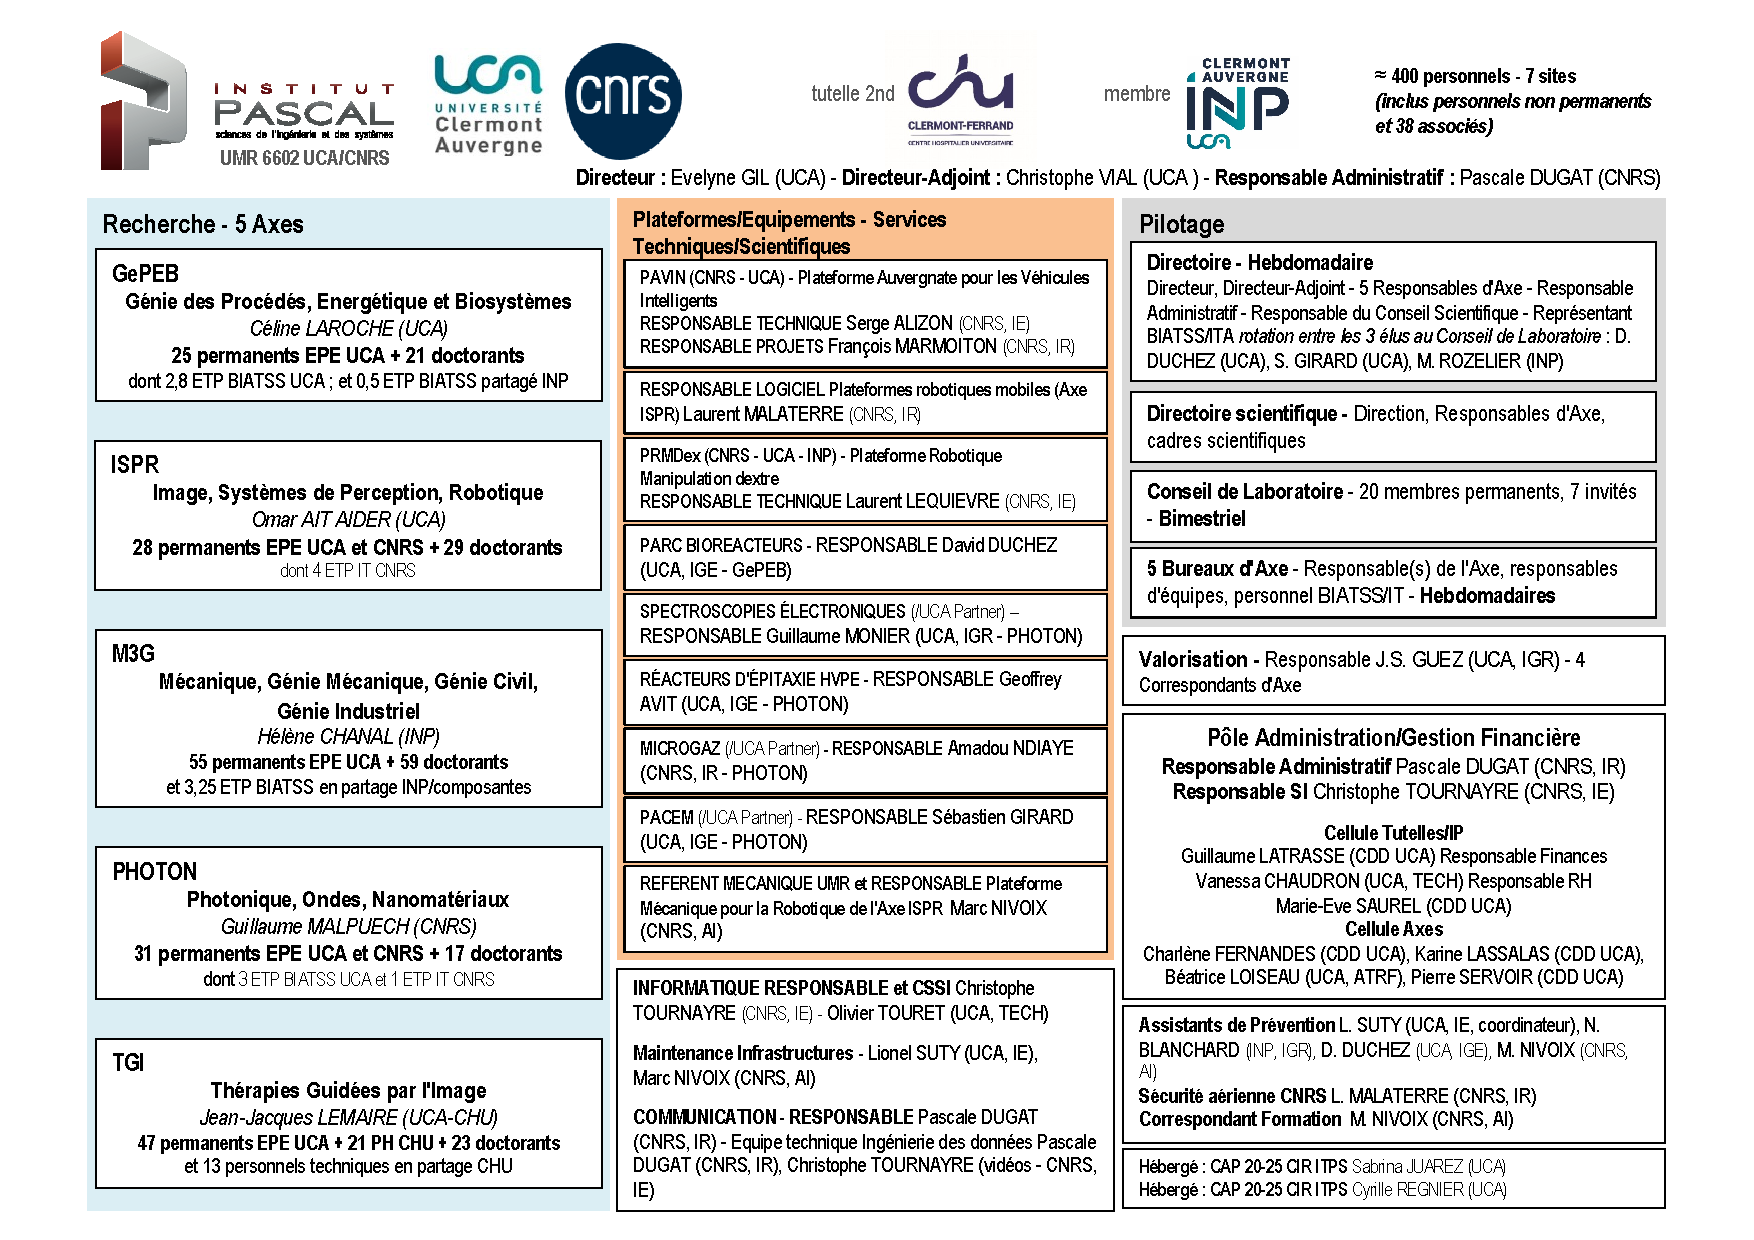
\includegraphics[width=1.1\textwidth]{img_pdf/organigramme_IP.pdf}}
    \caption{Organigramme structurel de l'Institut Pascal et de ses cinq axes de recherche}
    \label{fig:organigramme}
\end{figure}

\bigskip
\bigskip

Chaque axe regroupe un ensemble de personnels de recherche et d'appui dont la répartition globale fait l'objet de la section suivante.

\vspace*{\fill}

\clearpage
% ==============================================================================

% ==============================================================================
\section{Le service d'accueil}

Mon intégration dans une structure de recherche d'envergure impliquait de comprendre le fonctionnement quotidien de l'équipe et des infrastructures techniques.

\subsection{Gouvernance globale et environnement humain}
L'unité rassemble une communauté scientifique de près de 400 personnes caractérisée par une grande diversité de statuts. La répartition des effectifs met en évidence une forte composante académique et une dynamique d'encadrement importante :
\begin{itemize}[label=\textbullet]
    \item \textbf{Enseignants-chercheurs et chercheurs :} 137 enseignants-chercheurs (UCA, Clermont Auvergne INP), 5 chercheurs permanents CNRS, et 28 enseignants-chercheurs praticiens hospitaliers (UCA/CHU).
    \item \textbf{Personnels de santé et d'enseignement :} 23 praticiens hospitaliers (CHU) et 5 PRAG/PAST.
    \item \textbf{Personnels d'appui technique et administratif :} 11 ingénieurs et techniciens ITA (CNRS) et 15 personnels BIATSS (UCA).
    \item \textbf{Jeunes chercheurs et contractuels :} 147 doctorants et 28 contractuels à durée déterminée (CDD/Post-doc).
\end{itemize}

Au sommet de cette organisation, la direction générale de l'unité est assurée par \textbf{Mme Evelyne GIL} (Directrice), secondée par \textbf{M. Christophe VIAL} (Directeur Adjoint). La gestion opérationnelle et le secrétariat général sont coordonnés par \textbf{Mme Pascale DUGAT}, responsable administrative du site.

\subsection{L'Axe ISPR et l'équipe ComSee}
En parfaite adéquation avec la formation dispensée à l'EUPI, mon stage s'est déroulé au sein de l'axe \textbf{ISPR (Image, Systèmes de Perception, Robotique)}, sous la responsabilité scientifique de \textbf{M. Omar AIT AIDER}. L'activité de cet axe cible trois piliers scientifiques : l'image, la perception artificielle et la commande pour la robotique. 

Plus spécifiquement, l'intégration a eu lieu au cœur de l'équipe de recherche \textbf{ComSee} (contraction de \textit{COMputers that SEE}), dont les travaux s'articulent autour du domaine de la vision par ordinateur. Les activités de recherche de ComSee se concentrent sur deux thématiques principales qui croisent directement le sujet d'étude :
\begin{itemize}[label=\textbullet]
    \item \textbf{La vision géométrique :} Modélisation et étalonnage (calibration) de capteurs de vision (classiques, à obturateur roulant, plénoptiques), localisation et reconstruction 3D.
    \item \textbf{L'interprétation de séquences d'images :} Détection, reconnaissance et suivi d'éléments dans des séquences dynamiques, en utilisant des techniques d'apprentissage automatique (\textit{Machine Learning}) et de transfert d'apprentissage.
\end{itemize}

Les applications de cette équipe s'orientent vers les transports intelligents (navigation autonome de véhicules), la réalité augmentée, la vidéosurveillance et la vision robotique. Cette configuration offre un cadre idéal pour l'application concrète des concepts théoriques étudiés en Master 1.

\subsection{Environnement technique et plateformes d'expérimentation}
L'Institut Pascal se distingue par un écosystème technique exceptionnel composé de 7 plateformes expérimentales internes et 8 plateformes partenaires.\\
Il offre un appui unique pour la validation des travaux de recherche en ingénierie.\\

\bigskip

\textbf{Les plateformes majeures de l'axe ISPR :}\\
\hspace*{1cm} Pour les applications en automatique et en robotique, deux plateformes nationales de premier plan sont implantées sur les sites :
\begin{itemize}[label=\textbullet]
    \item \textbf{PAVIN (Plateforme Auvergnate Pour les Véhicules Intelligents / CNRS) :} \\
    \hspace*{.5cm} Dédiée à l'évaluation d'algorithmes de navigation, de perception et de commande en environnement routier urbain ou naturel simulé pour les véhicules autonomes.
    \item \textbf{PRMDex / ROBTOOL (EquipEx CNRS ROBOTEX) :}\\
    \hspace*{.5cm} Plateforme robotique de manipulation dextre et d'usinage robotisé.\\
    Elle est équipée de bras manipulateurs de haute précision, qui sont essentiels pour l'étude de l'interaction physique et de la commande d'outils complexes.
\end{itemize}

\bigskip

L'institut s'appuie également sur d'autres plateformes internes spécialisées comme la plateforme \textbf{PACEM} (Compatibilité Électromagnétique). De plus, la collaboration avec \textbf{Polytech Clermont} et \textbf{SIGMA Clermont} donne accès à des infrastructures partenaires d'essais mécaniques (\textbf{2MATech, MSGC}).\\

\bigskip
\bigskip

\textbf{Organisation et rythmes de travail :}\\
L'accueil et l'encadrement quotidiens étaient structurés pour simuler l'activité d'un ingénieur en recherche et développement au sein d'un laboratoire public.\\
Les modalités incluaient :
\begin{itemize}[label=\textbullet]
    \item \textbf{Le respect des horaires et présence sur site}\\
    \hspace*{.5cm} Le service fonctionne sur une base de présence en journée (généralement 9h00 - 18h00), rythmée par l'accès aux salles de développement informatique de l'équipe ComSee et aux plateformes robotiques.
    \item \textbf{Le suivi scientifique} \\
    \hspace*{.5cm} Des réunions de suivi et des séminaires d'axe permettent de faire régulièrement le point sur l'avancée de l'étude avec mes maîtres de stage, M.~\textbf{Thierry CHATEAU} et M.~\textbf{François MARMOITON}, afin de valider ou non les choix d'implémentation et de lever les verrous technologiques rencontrés.
\end{itemize}

% ==============================================================================
% DEUXIÈME PARTIE : LE POSTE OCCUPÉ ET L'ÉTUDE CONFIÉE
% ==============================================================================
\chapter{Présentation du poste occupé et de l'étude}

\section{Le poste occupé}

Dans le cadre de ce stage de Master~1 au sein de l'équipe \textbf{ComSee} de l'Institut Pascal, la fonction occupée a été celle d'un ingénieur stagiaire spécialisé dans le traitement de données et la vision par ordinateur.\\

\hspace*{.5cm}Elle s'insérait dans une recherche menée par l'Institut Pascal sur l'auto-calibration d'un système avec ses différents périphériques hétérogènes.\\

Sous l'encadrement de M. \textbf{Thierry CHATEAU} et de M. \textbf{François MARMOITON}, les missions quotidiennes confiées ont été construites autour de la manipulation, de l'extraction et du traitement de données complexes. \\

\hspace*{.5cm}Celles-ci provenaient des différents capteurs embarqués sur les plateformes expérimentales du laboratoire.\\

Cette intégration au sein du projet a permis d'établir un lien entre la recherche algorithmique\footnote{exploitation de modèles d'intelligence artificielle}, l'ingénierie des données nécessaires, et leur utilisation dans des conditions expérimentales réelles.\\
\hspace*{.5cm}Elle a ainsi conduit à concevoir, à développer et à tester différents pipelines de traitement de données en s'appuyant sur l'environnement \textbf{Linux}, notamment \textbf{Ubuntu}, ainsi que sur le middleware de robotique \textbf{ROS~2}.\\

Ce travail a été effectué en étroite collaboration avec un autre stagiaire de Master~2 en Automatique et Robotique, \textbf{M. Amadou BARRY}. \\
Notre complémentarité a permis de répartir efficacement les tâches du projet : 
\begin{itemize}[label=\textbullet]
    \item d'une part, le traitement des données en amont, destiné à améliorer les performances du modèle d'intelligence artificielle, qui fait l'objet de ce rapport ;\\
    \item d'autre part, le développement et l'optimisation du modèle d'IA, pris en charge par mon binôme.
\end{itemize}

\newpage

\section{L'étude confiée}

\hspace*{0.3cm}Les travaux menés au cours de ce projet s'inscrivaient dans le cadre des problématiques posées par la perception multi-capteurs et la navigation des véhicules autonomes.\\

\hspace*{.3cm}\textbf{L'objectif} était d'évaluer les possibilités d'auto-calibration extrinsèque des répères du système de vision d'un véhicule autonome,et des outils nécessaires à employer. Pour le déploiement du modèle d'apprentissage \textbf{VGGT}\footnote{Visual Geometry Grounded Transformer} qui a été étudié, en estimant \textbf{sa faisabilité, sa robustesse et sa pertinence}.\\

\textbf{En robotique mobile}, l'auto-calibration extrinsèque est fondamentale pour garantir la cohérence géométrique entre les différents capteurs embarqués.\\
Généralement, les méthodes classiques sont réalisées hors ligne à l'aide de mires géométriques fixes et dans des environnements contrôlés.\\
\hspace*{.5cm}L'auto-calibration vise à \textbf{estimer de manière autonome la pose relative entre les différents capteurs et le référentiel du véhicule}.\\

La plateforme mobile imposée pour les expérimentations était une navette autonome de type EasyMile EZ10.\\
\hspace*{.3cm} Cette dernière était équipée d’une caméra arrière monochrome ainsi que d’une autre caméra identique à l'avant, associées à deux caméras couleur disposées à l'avant, orientées respectivement vers la droite et vers la gauche.\\

Cette architecture présentait une limitation importante pour la réalisation du projet :\\

\hspace*{1cm}\textbf{Les caméras ne partageaient aucune zone de recouvrement visuel commune}.\\

\hspace*{.5cm}En complément, le véhicule embarquait deux LiDAR 3D à 360°, installés sur le toit, l’un à l’avant et l’autre à l’arrière, afin de fournir une perception géométrique 3D de l’environnement.\\


\begin{figure}[htbp]
    \centering
    \begin{minipage}{0.48\textwidth}
        \centering
        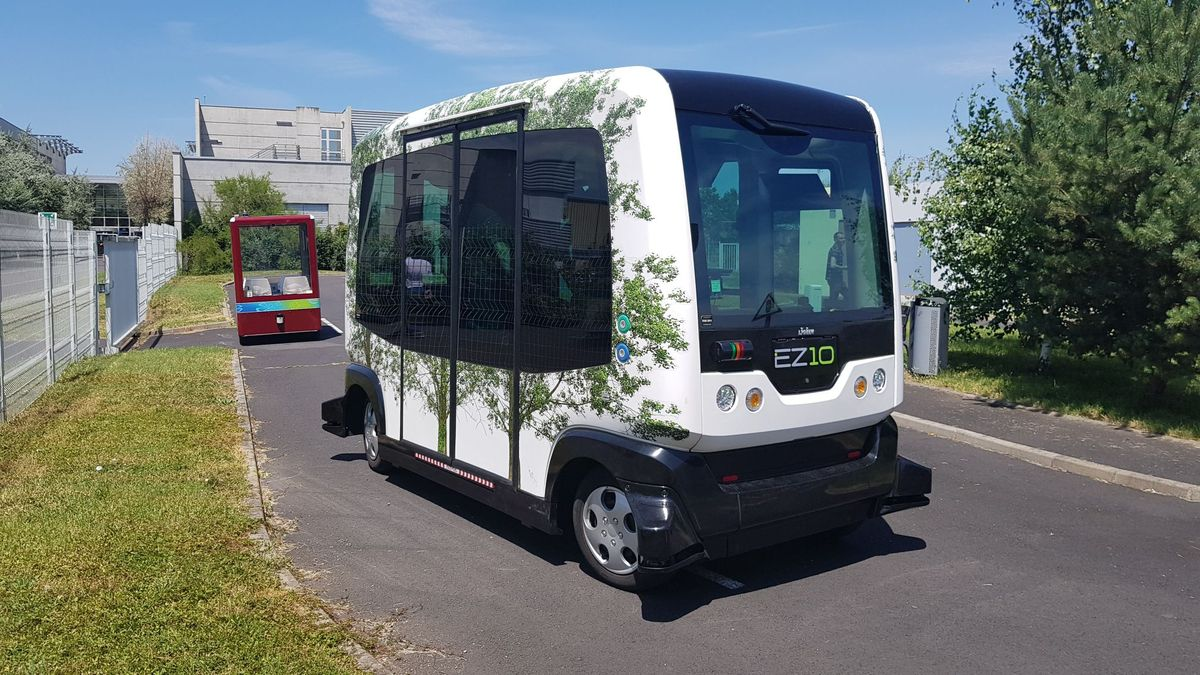
\includegraphics[width=\linewidth]{img_src/navette.jpg}
        \caption{Navette autonome EasyMile EZ10 utilisée lors des expérimentations.}
    \end{minipage}
    \hfill
    \begin{minipage}{0.48\textwidth}
        \centering
        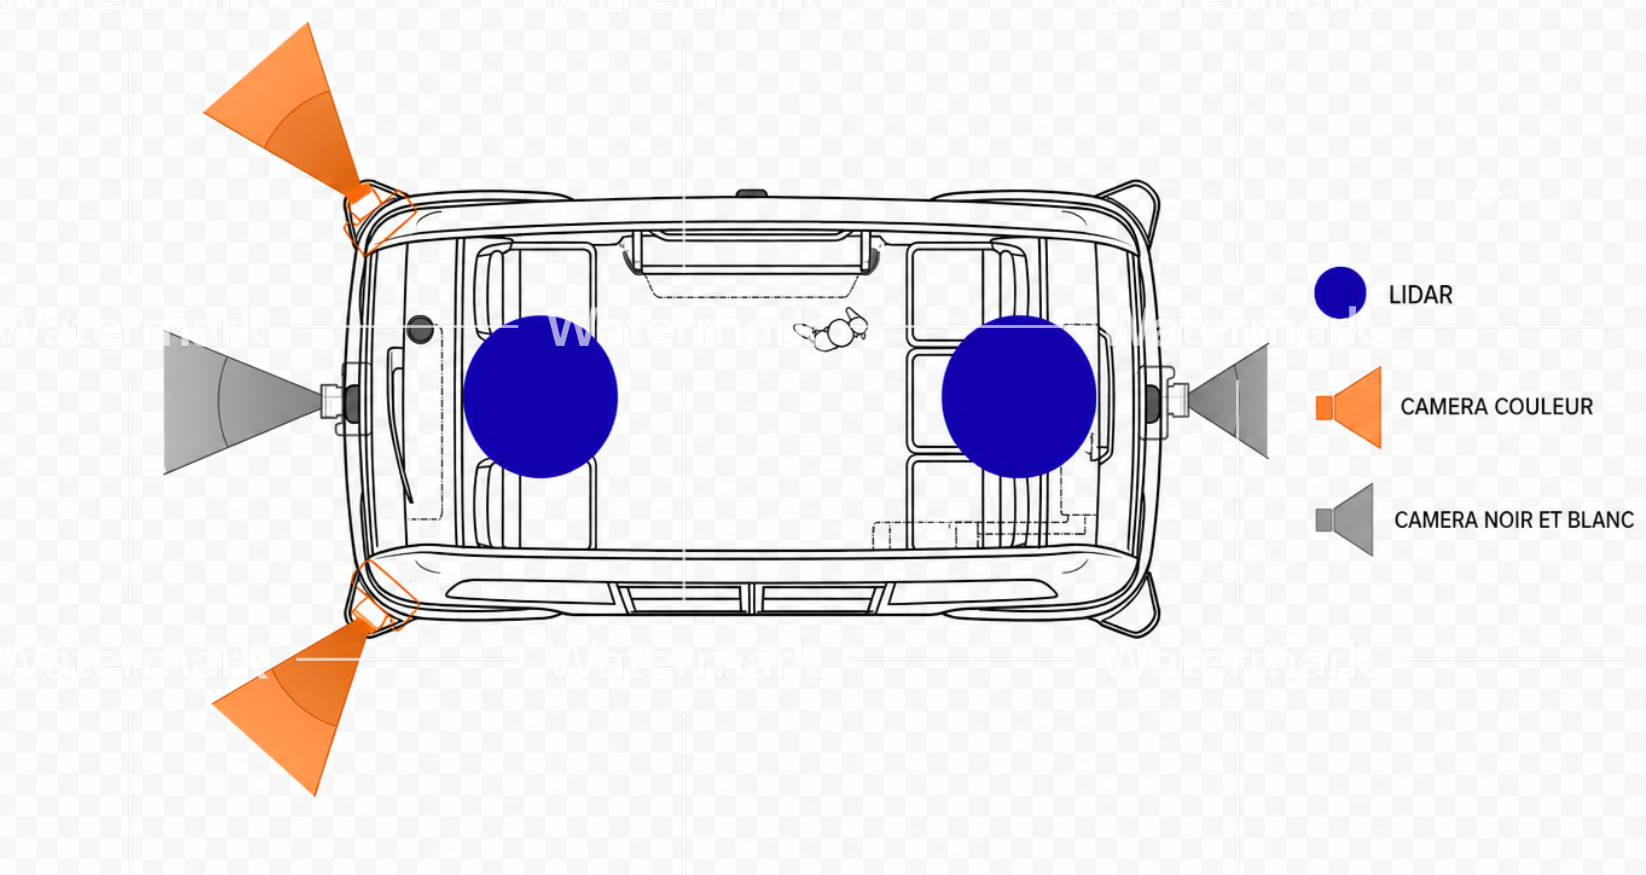
\includegraphics[width=\linewidth]{img_src/navelle_schéma.png}
        \caption{Schéma de l’architecture optique et des capteurs embarqués.}
    \end{minipage}
\end{figure}

\newpage

\vspace*{\fill}

\hspace*{.3cm}La configuration multi-capteurs hétérogènes imposée, bien que réaliste et représentative d’un véhicule autonome, constituait l’un des principaux défis du projet.\\
Elle limitait la redondance visuelle, nécessaire pour l’estimation robuste des poses et de la calibration extrinsèque.

\bigskip

Dans ce contexte, la réflexion c'est donc articulée autour de :\vspace{0.05cm}
\begin{itemize}[label=\textbullet]
    \item \textbf{L'ingénierie}
    \vspace{0.05cm}
    \item \textbf{La création d'un pipeline de traitement de données} 
\end{itemize}
\bigskip

\hspace*{.5cm}Les enregistrements \textbf{bruts} issus des différents capteurs physiques réels et stockés sous forme de fichiers \texttt{.rosbag}, nécessitaient la mise en place d'une chaîne de traitement capable d'alimenter efficacement un modèle d'IA spécialisé dans l'analyse géométrique.\\

\hspace*{.3cm}L'infrastructure nécessaire à l'extraction et à l'exploitation de ces différents flux de données a d'abord été conçue.\\
\hspace*{0.3cm}Plusieurs stratégies de pré-traitement numérique visant à améliorer la qualité des données transmises au modèle \textbf{VGGT} ont ensuite été proposées à l'ensemble de l'équipe, puis implémentées et évaluées.\\

\bigskip

\hspace*{.3cm}Celles-ci reposaient principalement sur le filtrage des données à partir de critères \textbf{cinématiques}, \textbf{temporels} et \textbf{visuels} définis préalablement, et sur l'exploitation des informations tridimensionnelles fournies par le LiDAR.\\
Les objectifs premiers étaient :\vspace{0.2cm}

\begin{itemize}[label=\textbullet]
    \item \textbf{limiter la redondance des données}
    \item \textbf{améliorer leur cohérence géométrique}
    \item \textbf{respecter les contraintes de calcul imposées par l'architecture du modèle}
\end{itemize}

\vspace{0.9cm}

\textsb{\hspace*{.3cm}Cette méthodologie a ainsi permis de construire progressivement un pipeline complet allant de l'extraction des données brutes issues de la plateforme expérimentale jusqu'à leur conditionnement pour l'analyse par le réseau \textbf{VGGT}, et de conserver les informations nécessaires à l'évaluation ainsi qu'à la validation des résultats obtenus.}

\vspace*{\fill}

\newpage

\chapter{Le démarrage de l'étude}

\section{Analyse et Critique préalables de l'existant}
\subsection{Analyse et Constat}
\vspace{0.5cm}
\hspace*{1em}Avant le début de ces travaux, le laboratoire disposait de jeux de données massifs enregistrés lors des circulations des véhicules autonomes sur la plateforme PAVIN. Ces données brutes, stockées sous forme de \texttt{.rosbag}, contenaient l'intégralité des flux non synchronisés : 
\vspace{.5cm}
\begin{itemize}
    \setlength{\itemsep}{1em}
    \renewcommand{\labelitemi}{{\large\bfseries\textbullet}}
    \item {\bfseries Les images issues des caméras embarquées (avant, arrière, gauche, droite)}
    \item {\bfseries Les nuages de points 3D générés par les LiDARs}
    \item {\bfseries Les informations de position et d'orientation du véhicule (odometry, GNSS, GPS)}
\end{itemize}
\bigskip
\hspace*{.5cm}Le point de départ algorithmique du modèle d'IA VGGT n'avait \textbf{aucun pipeline structuré} pour alimenter efficacement ce réseau avec des données pré-traitées, filtrées ou adaptées aux contraintes géométriques imposées par le modèle.

\subsection{Critique}
\vspace{0.5cm}
\begin{itemize}
    \setlength{\itemsep}{1.5em}
    \renewcommand{\labelitemi}{{\large\bfseries\textbullet}}
    \item {\bfseries Gourmandise computationnelle et contraintes de passage à l'échelle~: \vspace{0.3cm}} \\ 
    \hspace*{1em}Le modèle VGGT repose sur un mécanisme d'attention alternée (\textit{Frame-wise} et \textit{Global Attention}) appliqué à des \textit{tokens} visuels.\\
    \hspace*{.8cm} Si cette architecture offre d'excellentes capacités de prédiction géométrique directe (poses caméras, cartes de profondeur, \textit{point maps}), sa complexité mémoire (VRAM GPU) et les temps de calcul croissent de manière exponentielle avec le nombre d'images. \\

    \hspace*{1em}\textbf{Certaines contraintes matérielles (équipements informatiques, capacité de traitement) limitaient malheureusement l'échantillonnage de référence du modèle à seulement 20 images.} \\

\newpage
\vspace{4cm}

    \hspace*{1em}L'application directe de VGGT sur des séquences vidéo longues ou continues était donc impraticable sans un découpage strict en blocs (\textit{chunks}), introduisant inévitablement des dérives d'échelle et d'orientation cumulatives lors de la concaténation.
    
    \item {\bfseries Inadéquation des flux rosbags bruts et redondance sémantique~:  \vspace{0.3cm}}\\
    \hspace*{1em}Les enregistrements issus des véhicules autonomes (\texttt{.rosbag}) contiennent des données acquises à hautes fréquences. \vspace{0.05cm}

    \hspace*{.8cm}Dans des conditions réelles de circulation, le véhicule traverse régulièrement des phases d'arrêt (feux rouges, intersections) et de circulation très lente.\vspace{0.05cm}

    \hspace*{1em}Injecter ces images répétitives dans un réseau lourd comme VGGT provoque un gaspillage massif de ressources de calcul sans aucun gain géométrique, et peut induire le modèle en erreur sur des scènes statiques.\vspace{0.2cm}
    
    \item {\bfseries Hétérogénéité des modalités (2D visuel vs 3D LiDAR)~:  \vspace{0.3cm}} \\
    \hspace*{1em}Alors que le modèle VGGT travaille exclusivement sur l'information chromatique (RGB 2D), les véhicules autonomes disposent de LiDARs 3D qui fournissent une géométrie métrique absolue. \vspace{0.05cm}

    \hspace*{1em}\textbf{L'absence de passerelle(s) logicielle(s) }permettant de projeter ces nuages de points 3D sous forme de représentations denses 2D limite l'exploitation conjointe des capteurs.

\end{itemize}

\newpage

\section{Propositions de solutions}
\label{subsec:solutions_pipeline}


\setlength{\parskip}{0.5em}
\setlength{\parindent}{0pt}
\linespread{1.08}\selectfont

\hspace*{0.5cm} Les contraintes computationnelles du modèle VGGT et la nature brute des enregistrements, \texttt{nous ont amenés à nous réorienter vers une approche stratégique différente~:}

\textbf{Plutôt que d'appliquer l'IA de manière brute sur l'ensemble des données, il s'agissait d'optimiser l'alimentation du réseau avec un pré-traitement intelligent}.
\subsection{Pipeline de pré-traitement en amont}

\hspace*{0.5cm} \textbf{Les premières missions confiées }:
\begin{itemize}[label=\textbullet]
    \item \texttt{Comprendre le fonctionnement du pipeline de traitement de données existant}
    \item \texttt{Identification des principaux points de blocage liés à l'utilisation du modèle VGGT}
\end{itemize}

Elles ont permis de mettre en évidence un problème majeur :
\begin{itemize}[label=\textbullet]
    \item \textbf{Le modèle utilisé, sans aucune stratégie de sélection préalable issue des bases de données des caméras, ne pouvait pas être exploitable dans un contexte réel du véhicule autonome.}
\end{itemize}

\bigskip

\hspace*{.5cm}L'approche s'est avérée rapidement limitante par la création d'une forte redondance d'informations.\\
Elle générait une surcharge de calculs et pouvait nuire à \texttt{la fiabilité des prédictions géométriques}.\\

\hspace*{.5cm} Une solution a donc été proposée afin d'explorer la réduction du nombre d'images injectées dans le modèle sans perte d'informations utiles.\\
\hspace*{.5cm} L'analyse visuelle menée dans le cadre fixé par les responsables du stage a conduit à ne conserver que les vues qui présentaient un niveau de \textbf{saturation}, de \textbf{contraste} et de \textbf{flou} acceptable pour le modèle, tout en éliminant les images trop dégradées ou peu exploitables d'un point de vue géométrique.\\

\hspace*{.5cm} Le travail s'est ensuite concentré sur l'optimisation du filtrage visuel, afin de conserver les vues les plus exploitables, et de sélectionner celles où le véhicule était effectivement immobile. 
\begin{itemize}[label=\textbullet]
    \item \textbf{Images présentant un niveau de saturation, de contraste et de flou compatible avec l'estimation géométrique}
    \item \textbf{Vues acquises lorsque le véhicule était à l'arrêt, afin d'éviter les artefacts liés au mouvement}
\end{itemize}

Après plusieurs tests et analyses, il est apparu que le modèle ne pouvait pas fonctionner comme un simple système d'analyse d'images isolées et uniques.\\

\newpage

\vspace{5cm}

\subsection{Exploitation des données LiDAR}

\vspace{1cm}

\textsb{ Une piste importante du travail a consisté à exploiter les données LiDAR.} \vspace{0.1cm}

\hspace*{1cm} L'une des directives données consistait à chercher un moyen de \textbf{projeter les nuages de points 3D sur les images 2D}, afin de permettre la génération de cartes de profondeur et d'intensité, similaires aux images de caméra et exploitables par le modèle.\vspace{0.05cm}

\hspace*{.5cm} Ces cartes pouvaient ensuite être utilisées pour enrichir l'information visuelle et fournir au modèle des repères géométriques supplémentaires, facilitant ainsi l'estimation des poses et de la calibration extrinsèque.\vspace{0.1cm}

\hspace*{.5cm} Ensuite, toujours dans l'objectif d'obtenir des images 2D à partir des données LiDAR, l'utilisation d'une méthode de maillage (\textit{mesh}) appliquée au nuage de points 3D a été proposée. \vspace{0.05cm}

\hspace*{.5cm}L'objectif était de reconstruire une surface 3D en partant des points LiDAR, puis de projeter cette surface sur les images 2D pour générer des cartes de profondeur plus denses et continues.\\

\hspace*{.5cm} Les réflexions travaillées sur ces pistes et leurs développements ont amené à envisager une comparaison des prédictions du modèle avec une réalité terrain exploitable (en toute sécurité).\vspace{0.1cm}

\hspace*{.5cm}L'utilisation des données LiDAR et des algorithmes de SLAM a donc été proposée afin de générer des références métriques continues : \vspace{0.1cm}
\begin{itemize}[label=\textbullet]
    \item obtention d'une réalité terrain exploitable
    \item évaluation de la précision des poses estimées par VGGT
    \item évaluation de l'erreur de calibration extrinsèque
\end{itemize}

\newpage

\subsection{Sélection d'images et recouvrement visuel}

\hspace*{.5cm} Il a rapidement été constaté que le modèle VGGT ne se contentait pas d'analyser des images isolées, mais qu'il évaluait aussi la cohérence géométrique entre plusieurs vues successives.\\
\hspace*{.5cm}Le modèle s'appuyait sur des appariements visuels (\textit{feature matching}) entre les images pour estimer les poses relatives.\\
\hspace*{1cm}En fait, il évaluait largement le \textbf{recouvrement visuel} entre plusieurs vues temporellement décalées, ainsi que la quantité d'informations communes partagées.\\

\hspace*{1cm}Si le recouvrement était trop important, les images devenaient redondantes et le modèle consommait inutilement des ressources sans gain géométrique. \\
\hspace*{.3cm} À l'inverse, si celui-ci était trop faible, le lien géométrique entre les vues devenait insuffisant et la calibration devenait instable.

\paragraph{} 
Cette compréhension nous a conduit à proposer un module de sélection d'images adaptées aux besoins du modèle.\\

 L'objectif de ce module était de \textbf{récupérer une séquence d'images dont le taux de recouvrement était contrôlable et modulable} selon une consigne définie. \\
\hspace*{.3cm} Ainsi, sans envoyer l'ensemble des images d'une séquence, il devenait possible d'extraire un sous-ensemble d'images géométriquement cohérentes, optimisant l'alimentation du réseau et permettant une meilleure convergence du modèle.\\

 Ce module constituait une étape clé dans la chaîne de pré-traitement, permettant de \textbf{réduire le nombre d'entrées tout en conservant l'information essentielle} pour l'estimation de la calibration intrinsèque.

\bigskip
\bigskip
\bigskip

\begin{figure}[htbp]
    \centering
    \resizebox{\textwidth}{!}{%
    \begin{tikzpicture}[
        font=\small,
        node distance=1.9cm and 1.4cm,
        box/.style={draw=black, rounded corners=3pt, thick, align=center, minimum width=2.7cm, minimum height=1.0cm, fill=gray!8},
        select/.style={draw=black, rounded corners=3pt, thick, align=center, minimum width=3.4cm, minimum height=1.1cm, fill=green!12},
        ref/.style={draw=black, rounded corners=3pt, thick, align=center, minimum width=2.8cm, minimum height=1.0cm, fill=blue!8},
        arrow/.style={->, >=latex, thick}
    ]
        \node[box] (raw) {Données brutes\\\texttt{.rosbag}};
        \node[box, right=1.6cm of raw] (sync) {Synchronisation par\\correspondance temporelle};
        \node[box, right=1.6cm of sync] (kin) {Filtrage cinématique\\(arrêt du véhicule)};
        \node[box, right=1.6cm of kin] (vis) {Filtrage visuel\\(contraste, flou, saturation)};

        \node[box, below=1.7cm of vis] (match) {Appariement LoFTR\\et recouvrement visuel};
        \node[select, below=1.7cm of kin] (sel) {Sous-séquence retenue\\recouvrement contrôlé};
        \node[box, below=1.7cm of raw] (out) {Entrées VGGT\\sélectionnées};
        \node[ref, left=1.8cm of sel] (refbox) {LiDAR + SLAM\\référence géométrique};

        \draw[arrow] (raw) -- (sync);
        \draw[arrow] (sync) -- (kin);
        \draw[arrow] (kin) -- (vis);
        \draw[arrow] (vis) -- (match);
        \draw[arrow] (match) -- (sel);
        \draw[arrow] (refbox) -- (sel);
        \draw[arrow] (sel) -- (out);
    \end{tikzpicture}
    }
    \caption{Schéma récapitulatif du pipeline de sélection d'images appliqué avant l'alimentation de VGGT.}
\end{figure}

\newpage

\chapter{Étude : Mise en place et suivi des solutions proposées}

\section{Cadre expérimental}

Le cadre expérimental de cette étude visait à éprouver \textbf{la robustesse du modèle d'IA VGGT} face aux contraintes géométriques réelles d'un véhicule autonome en mouvement.\\

\hspace*{.3cm} Deux validations numériques et algorithmiques ont été conduites à partir d'enregistrements de données standardisées (\texttt{rosbag}) capturées sur la plateforme d'expérimentation \textbf{PAVIN}.\\

Les scénarios sélectionnés simulaient une cinématique hautement dynamique :
\begin{itemize}[label=\textbullet]
\item le parcours du périmètre du site PAVIN ;
\item la gestion d'un carrefour à sens unique (rond-point).
\end{itemize}

\bigskip
\bigskip

\begin{figure}[htbp]
\centering
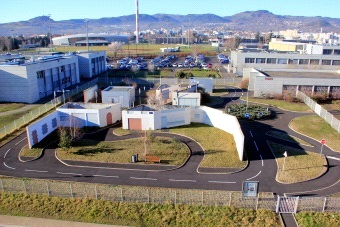
\includegraphics[width=0.7\linewidth]{img_src/PAVIN.jpg}
\caption{Plateforme d'expérimentation PAVIN située à Aubière}
\label{fig:pavin}
\end{figure}

\newpage

\subsection{Scénario retenu}
\paragraph{}
Au cours du stage, le scénario de la gestion d'un carrefour à sens unique a finalement été privilégié.\\
\hspace*{.5cm}Ce choix a été dicté par les résultats obtenus lors des expérimentations. En effet, les configurations plus exigeantes n'ont pas permis d'obtenir à partir de VGGT une réalité terrain stable et cohérente.\\

\hspace*{.5cm}\textbf{Les sorties du modèle ne pouvaient alors être évaluées de manière fiable que par un regard subjectif, fondé sur une interprétation visuelle des résultats, sans mesure quantitative de référence.\\}

\hspace*{.5cm}Cette limite a renforcé l'idée qu'il fallait privilégier un cas d'étude suffisamment représentatif du comportement réel du système, tout en restant exploitable pour une évaluation objective.

\vspace{0.5cm}

\begin{figure}[htbp]
\centering
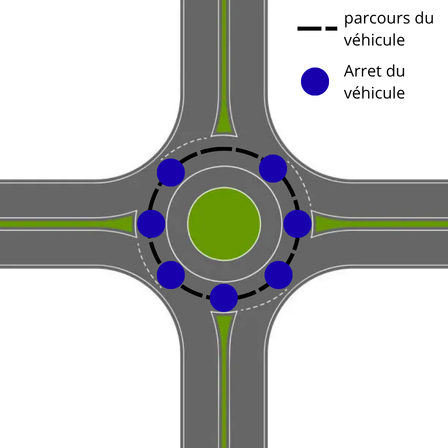
\includegraphics[width=0.5\linewidth]{img_src/parcours_du_vehicule.png}
\caption{Parcours du véhicule avec l'arret}
\label{fig:pavin}
\end{figure}

\vspace{0.2cm}

\hspace*{.5cm}Le scénario du rond-point a été retenu pour soumettre les modèles d'apprentissage profond à des contraintes fortement non linéaires, tout en offrant un cadre de navigation maîtrisé et représentatif pour l'évaluation des performances.

\newpage

\vspace{1cm}

\textbf{\hspace*{0.3cm} L'hypothèse sous-jacente a ce choix de trajectoire était double :}\vspace{0.05cm}

\begin{itemize}[itemsep=0.5em, label=\textbullet, leftmargin=1.5cm]
    \item \textbf{Garantie de généralisation :}\vspace{0.02cm}

    \hspace*{0.5cm}Un environnement curviligne et changeant (le rond-point) pouvait induire des variations continues de l'orientation des caméras, de la parallaxe et du champ visuel global.\\
    \hspace*{0.4cm}Si le réseau était capable de converger et d'estimer une auto-calibration intrinsèque stable dans ces conditions critiques, sa capacité de généralisation était implicitement validée pour des trajectoires rectilignes ou des scénarios autoroutiers plus simples, alors que la réciproque n'est pas forcément vraie.

    \item \textbf{Sollicitation cinématique :}\vspace{0.02cm}

    \hspace*{0.5cm}Le mouvement de rotation continue autour du centre du rond-point permettait de valider le comportement du modèle face à des couplages de mouvements complexes (translations latérales et rotations simultanées).
\end{itemize}

\vspace{0.1cm}

\hspace*{1cm}La séquence d'enregistrement a débuté en amont du rond-point par une phase stationnaire d'une durée calibrée d'environ 15 secondes.\\
 Cet arrêt initial n'était pas un artefact d'enregistrement, mais une phase de contrôle volontaire.\vspace{0.1cm}

\hspace*{.5cm}Elle permettait de constituer une ligne de base (\textit{baseline}) d'images de référence les plus nettes possible, exemptes de flou cinétique, offrant ainsi des conditions idéales pour le traitement des données obtenues.

\subsection{Logistique utilisée}

\begin{itemize}[itemsep=0.2em, leftmargin=2cm, label=\textbullet]

    \item \textbf{Perception optique périphérique :} \\
    \hspace*{0.5cm}Quatre caméras couvrant l'espace périphérique du véhicule : deux caméras monochromes (avant et arrière) et deux caméras couleur (avant-droite et avant-gauche), fournissant la matière première bidimensionnelle au réseau VGGT.

\begin{figure}[htbp]
    \centering
    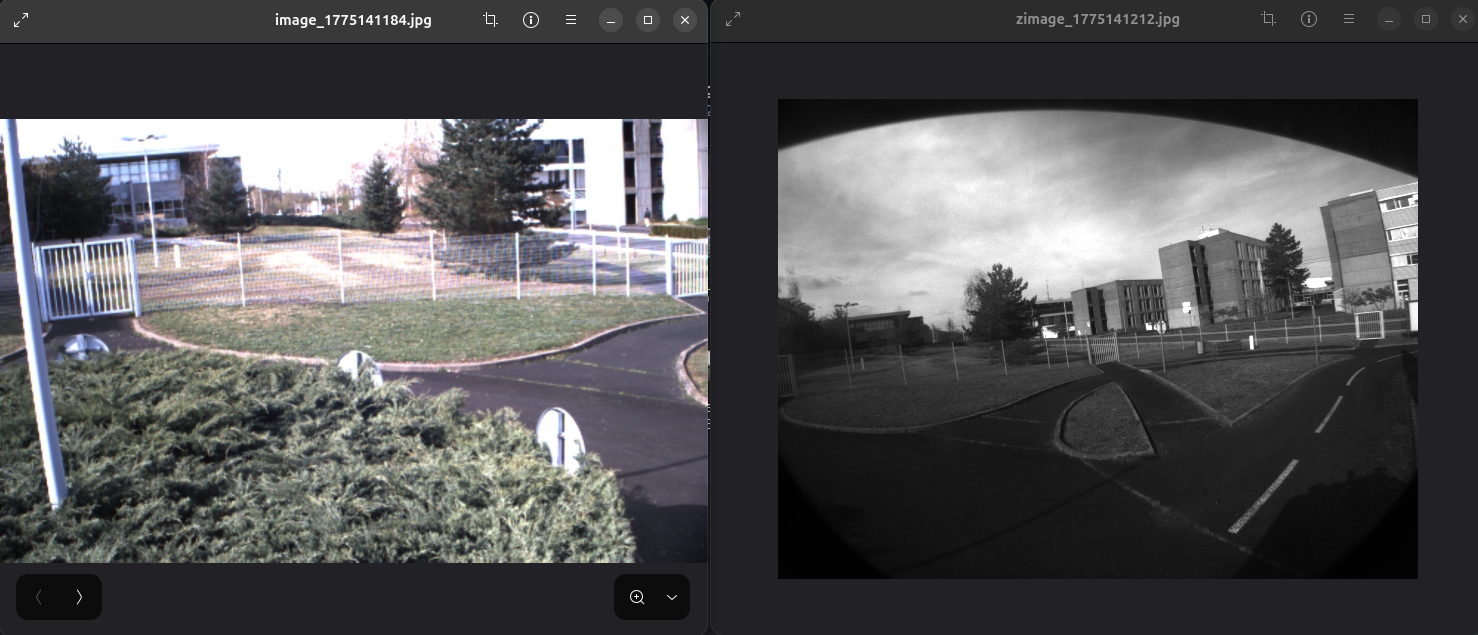
\includegraphics[width=0.8\textwidth]{img_src/image_source.png}
    \caption{Exemples d'images acquises par les caméras embarquées}
    \label{fig:images_sources_camera}
\end{figure}

\newpage

    \item \textbf{Perception télémétrique 3D :}\\
    \hspace*{1cm}Deux capteurs LiDAR 3D (\textbf{Hesai Pandar XT32}) disposés de part et d'autre des essieux avant et arrière, fournissant les nuages de points de l'environnement.

\begin{figure}[htbp]
    \centering
    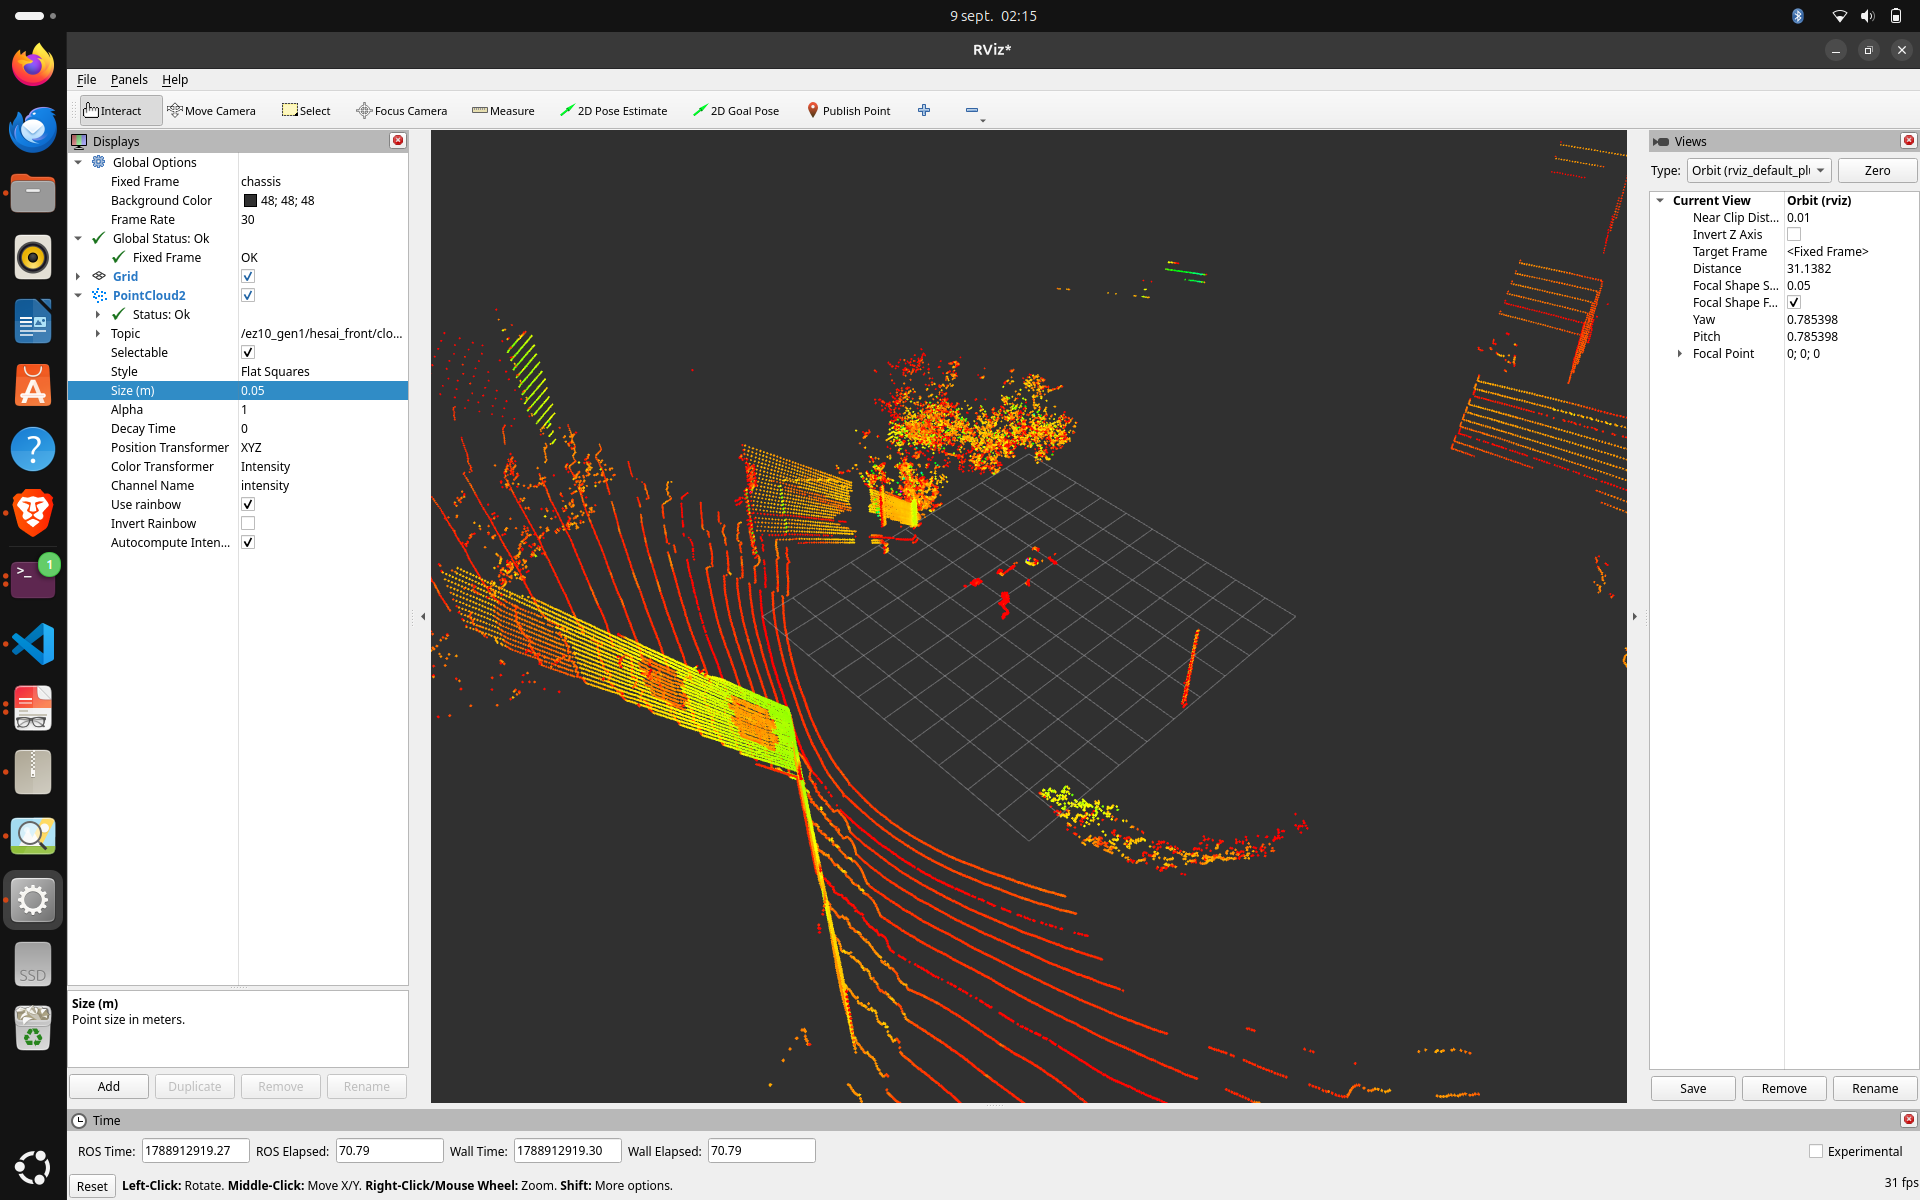
\includegraphics[width=0.7\textwidth]{img_src/rviz2_lidar.png}
    \caption{Exemple d'acquisition par un capteur LiDAR}
    \label{fig:images_sources_lidar}
\end{figure}


    \item \textbf{Localisation absolue :}\\
    \hspace*{1cm}Un récepteur GNSS (GPS) fournissait la pose tridimensionnelle géoréférencée du véhicule servant de base pour l'établissement de la vérité terrain.

    \item \textbf{Odométrie proprioceptive :} \\
    \hspace*{1cm}Les données d'état cinématique issues des encodeurs du châssis à quatre roues directrices (\textit{Four-Wheel Steering} -- 4WS), indispensables pour caractériser dynamiquement les déplacements du porteur.

\begin{figure}[htbp]
    \centering
    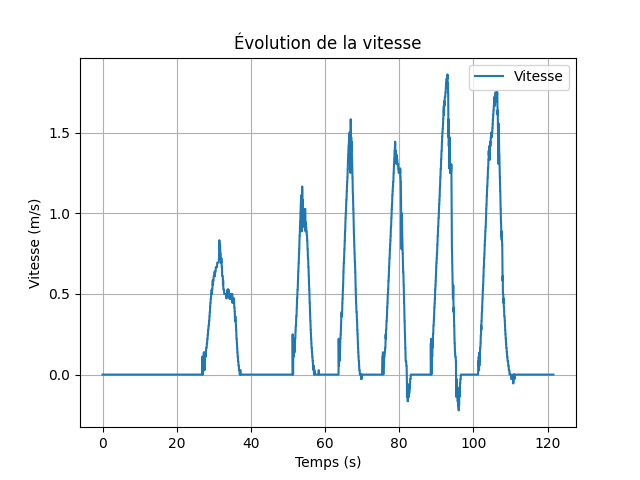
\includegraphics[width=0.6\textwidth]{img_src/vitesse_odom.png}
    \caption{Graphique de l'évolution de la vitesse du véhicule, mesurée par les capteurs d'odométrie}
    \label{fig:images_sources_odom}
\end{figure}

\end{itemize}

\clearpage

\section{Filtrage cinématique (à l'arrêt du véhicule)}

\subsection{Synchronisation temporelle stricte et gestion des flux intermittents}

\hspace*{1cm}La décompression du fichier \textit{rosbag} donnait la possibilité d'isoler l'accès aux flux des quatre caméras périphériques.\vspace{0.1cm}

\hspace*{.5cm}La première étape indispensable a consisté pour réaliser une synchronisation temporelle rigoureuse de ces images.\vspace{0.1cm}

\hspace*{.5cm}En effet, lors du lancement d'un enregistrement sous l'architecture ROS, la souscription et la capture effective des données de chaque nœud capteur ne débutaient pas de manière strictement simultanée.\vspace{0.1cm}

\hspace*{1cm}C'est pour cette raison qu'un temps de calibration a été prévu chaque début d'enregistrement, pour garantir que les flux d'images présentent, à un moment donné, un alignement temporel.

\bigskip

\begin{figure}[htbp]
    \centering
    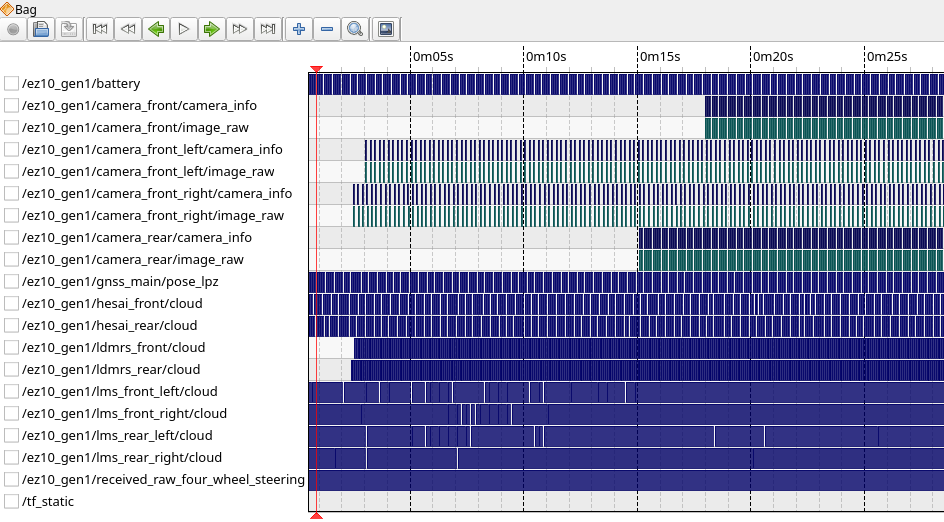
\includegraphics[width=0.9\textwidth]{img_src/robag_rqt.png}
    \caption{Représentation des flux de données de tous les périphériques, visualisés dans l'environnement RQT\_graph}
    \label{fig:images_aff_rosbags}
\end{figure}

\vspace{1cm}

\hspace*{1cm}Pour y remédier, un algorithme d'appariement basé sur une fenêtre temporelle glissante, développé en langage Python, a été utilisé. \\
L'objectif était de surveiller les estampilles temporelles (\textit{timestamps}) de chaque image reçue et d'associer celles dont l'écart temporel était inférieur à un seuil critique fixé à 1~ms. 

\newpage

\hspace*{1cm}Afin de garantir l'intégrité de la géométrie de reconstruction, le script appliquait une politique de filtrage stricte à chaque instant $T$.\vspace{0.1cm}

\hspace*{.5cm} Si l'une des quatre caméras présentait une perte de trame (\textit{frame drop}) ou un retard de publication, le groupe d'images incomplet était systématiquement rejeté du pipeline.\vspace{0.1cm}

\hspace*{1cm} Bien que cette exclusion stricte réduise le volume total des données et puisse théoriquement impacter la densité spatiale de l'échantillonnage, ce choix a été ici pleinement justifié.\vspace{0.05cm}

\begin{itemize}[itemsep=0.5em]
	\item D'une part, la phase d'arrêt de 15 secondes planifiée lors de l'acquisition offrait une redondance temporelle suffisante pour compenser ces pertes.
	\item D'autre part, le modèle VGGT était particulièrement lourd et consommateur en ressources de calcul, ce qui nous limitait à 20 images et rendait la qualité et la complétude de la synchronisation prioritaires sur la quantité de données.
\end{itemize}

\bigskip


\subsection{Extraction et tri odométrique }

\vspace{1cm}

\hspace*{1cm}Une fois le script Python exécuté, les quadruplets d'images parfaitement synchronisés ont été répartis dans quatre répertoires distincts correspondant à chaque caméra.\vspace{0.1cm}

\hspace*{0.5cm}L'étape suivante a été le filtrage automatique des phases stationnaires.\vspace{0.05cm}

\hspace*{1cm} En exploitant les données odométriques issues du châssis cinématique à quatre roues directrices (4WS), l'algorithme devait isoler les séquences où le véhicule présentait une vitesse linéaire nulle.\vspace{0.1cm}

\hspace*{0.5cm}Un premier script Python a donc été développé afin d'extraire les données d'odométrie et de les analyser pour identifier les périodes d'immobilité.\\
\hspace*{0.5cm}Il a ensuite suffi de créer un second script pour extraire les images des caméras à partir des timestamps où le véhicule était à l'arrêt.\\

\hspace*{1cm} Pour s'affranchir du bruit des mesures des capteurs odométriques embarqués, un seuil de tolérance minimal, proche de zéro, a été configuré afin de valider mathématiquement l'état d'immobilité. Lors des expérimentations, ce seuil a permis de détecter précisément les instants où le véhicule était effectivement à l'arrêt.\\

\newpage

\hspace*{1cm}À l'issue de ce pipeline de pré-traitement, les images filtrées ont été soumises au modèle VGGT. Le choix de privilégier des scènes fixes répondait à une double contrainte scientifique :\vspace{0.05cm}

\begin{itemize}
    \item \textbf{Élimination du flou cinétique :}\vspace{0.05cm}

 \hspace{1cm}L'immobilité du véhicule devait garantir des contours nets sur les objets de l'environnement.\vspace{0.05cm}
 
 \hspace{0.5cm}Il était attendu que cela facilite la convergence des convolutions du réseau de neurones.
    
\end{itemize}

\vspace{0.5cm}

\hspace*{1cm} À la fin de ce module, une analyse critique des données a mis en évidence deux limitations majeures des capteurs: \vspace{0.05cm}

\begin{itemize}[label=\textbullet, itemsep=0.3cm]
    \item \textbf{Distorsion optique :}\vspace{0.05cm}

 \hspace{0.5cm}Les objectifs des caméras avants et arrières présentaient des distorsions géométriques notables (effet grand angle / \textit{fisheye}). Un étalonnage intrinsèque (correction de distorsion) s'avérait donc nécessaire pour ne pas fausser l'analyse géométrique du modèle d'IA.

    \item \textbf{Sensibilité aux conditions lumineuses :}\vspace{0.05cm}

 \hspace{0.5cm}Selon l'orientation du véhicule par rapport au soleil, certaines images souffraient d'un phénomène de saturation (surexposition), les rendant problématiques pour leur exploitation. Un filtrage basé sur l'histogramme de luminance devait être envisagé pour écarter automatiquement ces trames saturées.

\end{itemize}

\vspace{1cm}

\textbf{\hspace{1cm}Ce constat nécessitait l'introduction d'un post-traitement d'images.}

\newpage

\section{Amélioration de la Qualité des Images}

\subsection{Traitement de la distorsion optique}

\paragraph{}
La distorsion (souvent de type \textit{fisheye} ou \textit{barrel distortion}) n'est pas un défaut involontaire, mais un compromis optique assumé pour maximiser le champ de vision (FOV - Field of View).

\begin{itemize}[itemsep=1.5em]
    \item \textbf{Champ de vision ultra-large ($180^\circ$ à $220^\circ$) :}\\

    \hspace*{1cm} Pour des applications de suivi d'environnement, d'odométrie visuelle ou de SLAM, une seule caméra grand-angle permet de couvrir à la fois les angles morts latéraux et la zone frontale du véhicule.\\
    Cela évite de multiplier le nombre de caméras embarquées tout en conservant une couverture spatiale suffisante pour les algorithmes de reconstruction et d'estimation de pose.

    \item \textbf{Corrigible mathématiquement :}\\

    \hspace*{1cm} Contrairement au flou de mouvement ou au bruit numérique, la distorsion optique géométrique est \textbf{déterministe}.\\
    Elle se modélise précisément via un étalonnage intrinsèque (par exemple un modèle à division ou un modèle omnidirectionnel de type Scaramuzza / Mei).\\

    \hspace*{1cm} Une fois la caméra calibrée, on peut projeter de façon inverse les coordonnées image 2D déformées vers l'espace 3D à l'aide des paramètres intrinsèques et des coefficients de distorsion, sans perte d'information utile pour la reconstruction géométrique.
\end{itemize}

\paragraph{}
Dans notre pipeline, la correction est effectuée en amont de l'appariement visuel : les paramètres issus du topic \texttt{camera\_info}\footnote{message ROS2 contenant les paramètres d'étalonnage (calibration) et les métadonnées d'une caméra} sont utilisés pour redresser les images avant toute étape d'extraction de caractéristiques ou d'appariement dense.\\

\hspace*{.5cm} Le modèle unifié de Mei (Unified Camera Model), adapté aux objectifs très grand‑angle / fisheye, a ensuite été retenu. Le principe est un mapping inverse : pour chaque pixel de l'image rectifiée on calcule d'abord un vecteur directionnel 3D, on le projette sur la sphère unité, on applique le paramètre de distorsion $\xi$, puis on reprojette dans l'image brute pour effectuer un remap.\\

\newpage



\begin{enumerate}[label=\arabic*) , leftmargin=0pt]
\item \textbf{Définition du plan virtuel corrigé à partir de la grille $(u_{\text{new}},v_{\text{new}})$ on construit :}\\

\texttt{\[
X=\frac{u_{\text{new}}-c_x}{f_x\cdot\text{zoom}},\quad Y=\frac{v_{\text{new}}-c_y}{f_y\cdot\text{zoom}},\quad Z=1.
\]}

\bigskip

\item \textbf{Projection sur la sphère normalisation $\rho=\sqrt{X^2+Y^2+Z^2}$ et}\\

\texttt{\[
X_s=\frac{X}{\rho},\quad Y_s=\frac{Y}{\rho},\quad Z_s=\frac{Z}{\rho}.
\]}

\bigskip

\item \textbf{Application de la distorsion ($\xi$) on décale le centre de projection :}\\

\texttt{\[
x_m=\frac{X_s}{Z_s+\xi},\quad y_m=\frac{Y_s}{Z_s+\xi}
\]}
\bigskip

(on peut ajouter $1\mathrm{e}{-6}$ au dénominateur pour la stabilité).\\


\bigskip

\item \textbf{Reprojection dans l'image source avec la matrice intrinsèque $K$ :}

\texttt{\[
map_x=f_x\cdot x_m + c_x,\quad map_y=f_y\cdot y_m + c_y.
\]}
\end{enumerate}

\noindent\textbf{ 5) Reconstruction par interpolation (avec la librairie OpenCV) on applique :}

\begin{center}
\texttt{cv2.remap(map\_x, map\_y, INTER\_LINEAR)}
\end{center}
pour lire les couleurs dans l'image brute en utilisant ces cartes flottantes. 

\bigskip
\bigskip
\bigskip

\hspace*{.5cm} Après cette étape, les images sont redressées et prêtes pour l'appariement visuel et l'estimation de la calibration. \\
Évidemment, cette correction provoque un recadrage et une perte de pixels sur les bords, mais elle est indispensable pour garantir la cohérence géométrique des correspondances entre vues.


\newpage

\subsection{Traitement de la saturation}
\paragraph{}
La saturation (ou \textsb{« brûlage »}) survient lorsque l'éclairement incident dépasse la plage dynamique du capteur ; les photosites atteignent leur valeur maximale et l'information des hautes lumières est irrémédiablement perdue. \vspace{0.1cm}

\hspace*{1cm} Dans ce projet, la quantification de cet effet a été réalisée par le calcul de la proportion de pixels dont l'intensité atteint la valeur maximale du codage (255 en image 8 bits). Ce test a été exécuté en prétraitement pour identifier et rejeter les trames dont une portion significative de la dynamique est perdue.\vspace{0.05cm}

\begin{enumerate}[label=\arabic*),leftmargin=2cm]
    \item On construit un masque bool\'een \texttt{mask = (img\_gray == 255)} valant \texttt{True} uniquement pour les pixels satur\'es ($255$).
    \item On calcule $N_{\text{satur\'es}} = \texttt{np.sum(mask)}$, le nombre total de pixels satur\'es.
    \item On normalise par la surface totale $N_{\text{total}}$ pour obtenir :
    \[
    \text{Ratio} = \frac{N_{\text{satur\'es}}}{N_{\text{total}}}
    \]
\end{enumerate}

\hspace*{1cm} Cette proportion fournit une mesure simple et robuste de la surface « brûlée » de l'image et sert, si elle dépasse un seuil fixé, à rejeter la trame avant l'appariement visuel.

\hspace*{1cm} Dans le pipeline développé, le seuil de tolérance retenu est de $15\%$ de pixels saturés. Cette valeur empirique a été choisie après analyse des performances du modèle \textbf{VGGT} sur le jeu de données de l'étude.\vspace{0.05cm}

\subsection{Traitement du contraste}

\hspace{1cm}Dans ce projet, nous avons observé que certaines images présentaient des aplats (tout noir, tout blanc ou gris uniforme) traduisant un faible contraste.\\
Un contraste insuffisant réduit la quantité d'informations locales exploitables pour l'appariement et la calibration.\vspace{0.1cm}

\hspace{1cm}Si tous les pixels ont la même valeur ($x_i = \mu$ pour tout $i$), alors $\sigma=0$. Un $\sigma$ très faible indique un manque de contraste. Dans ce pipeline de prétraitement, nous avons rejeté les images dont $\sigma < 5$ (seuil empirique pour images 8 bits), car elles apportaient peu d'informations géométriques au modèle.\vspace{0.05cm}

\textbf{Calcul de l'écart-type du contraste :}
L'écart-type $\sigma$ mesure la dispersion des valeurs des pixels autour de la moyenne $\mu$ de l'image :
\[
\sigma = \sqrt{\frac{1}{N} \sum_{i=1}^{N} (x_i - \mu)^2}
\]
où :
\begin{itemize}
    \item $x_i$ : valeur du pixel $i$,
    \item $\mu$ : valeur moyenne de tous les pixels,
    \item $N$ : nombre total de pixels (\texttt{img\_gray.size}).
\end{itemize}

\newpage

\subsection{Traitement du flou}

\vspace{1cm}

\paragraph{}
Dans ce projet, le test de flou a identifié l'absence de contours nets dans l'image. Une image bien focalisée présente des transitions d'intensité abruptes sur les bords des objets ; le flou lisse ces transitions.

\paragraph{}
On a déterminé : \vspace{0.05cm}
\begin{itemize}[itemsep=1em]
    \item une image comme nette si la variance du Laplacien est élevée (ex. $>100$ sur images 8 bits)
    \item une image comme floue si la variance est faible (ex. $<15$), auquel cas la trame est rejetée en prétraitement.
\end{itemize}

\vspace{0.5cm}

\hspace*{1cm} Bien évidemment, ces seuils sont empiriques et peuvent être ajustés selon les besoins du projet et la sensibilité du modèle VGGT aux variations de netteté. \vspace{0.05cm}

\hspace*{0.5cm}Mais les seuils choisis ont été validés par des tests sur notre jeu de données, en comparant visuellement les images rejetées avec celles conservées.\vspace{1cm}

\textbf{Calcul de la variance du Laplacien :}\\
On applique d'abord l'opérateur Laplacien pour extraire la dérivée seconde spatiale de l'image :
\[
\Delta I = \frac{\partial^2 I}{\partial x^2} + \frac{\partial^2 I}{\partial y^2}
\]

\vspace{1cm}

\hspace{0.5cm}Ensuite on calcule la variance des valeurs du Laplacien sur l'image : une variance élevée indique la présence de contours marqués, une variance faible indique une image floue.


\newpage

\section{Génération d'images à partir du LiDAR 3D}

\hspace*{0.3cm} \textit{L'objectif de cette deuxième approche consistait à exploiter la complémentarité géométrique entre les capteurs proprioceptifs et extéroceptifs afin de générer une référence de vérité terrain (\textit{Ground Truth}) tridimensionnelle suffisamment précise pour servir de référence lors de la phase d'auto-calibration.}\\

\hspace*{0.3cm}Cette approche constituait une proposition d'exploitation des données LiDAR. L'idée était de comparer une reconstruction tridimensionnelle obtenue à partir du LiDAR et d'un algorithme de SLAM avec la reconstruction prédite par le modèle \textbf{VGGT}. Une telle comparaison aurait permis d'évaluer les résultats du réseau à partir d'une référence géométrique indépendante des seules données visuelles.\\

\hspace*{0.3cm}Cependant, cette méthode n'a pas pu être menée à son terme dans le cadre matériel disponible. Le véhicule ne disposait pas de l'ensemble des équipements nécessaires pour garantir une acquisition et une synchronisation suffisamment adaptées à la reconstruction LiDAR-SLAM. Les essais réalisés n'ont donc pas permis d'obtenir une référence tridimensionnelle suffisamment fiable pour effectuer une comparaison quantitative avec VGGT. Cette piste reste en cours de recherche et pourra être poursuivie avec les moyens matériels disponibles ou avec une instrumentation plus adaptée.

\subsection{Développement d'un algorithme SLAM personnalisé}

\hspace*{.3cm}Afin d'appréhender finement les mécanismes de fusion des différentes sources de données, sans dépendre directement d'une architecture considérée comme une « boîte noire », un premier pipeline de SLAM (\textit{Simultaneous Localization and Mapping}) spécifique a été envisagé à partir des données extraites du \texttt{rosbag}.\\

\hspace*{.3cm}Le pipeline devait s'appuyer sur la combinaison de plusieurs sources d'informations complémentaires :
\begin{itemize}[label=\textbullet]
    \item\textbf{L'odométrie cinématique} issue du châssis à quatre roues directrices (4WS)
    \item\textbf{Les informations géospatiales absolues} fournies par le récepteur GNSS (GPS),
    \item\textbf{Les scans tridimensionnels bruts} acquis par le LiDAR 3D \textbf{Hesai Pandar XT32}.
\end{itemize}


\newpage

\subsection{Déploiement d'une architecture SLAM}

\hspace*{1cm}Dans une démarche de recherche visant à comparer l'approche envisagée avec une solution existante validée, une seconde architecture de SLAM tridimensionnelle a été étudiée sous l'environnement ROS~2.\vspace{0.05cm}

\hspace*{1cm}Le choix s'est porté sur le framework open-source \textbf{Kitware LiDAR SLAM}, intégré au système à travers le package \textit{lidar\_slam}.\vspace{0.05cm}

\hspace*{0.5cm}Cette seconde implémentation devait permettre de disposer d'un point de comparaison (\textit{benchmark}) pour évaluer les résultats du pipeline de SLAM personnalisé envisagé en amont.\vspace{0.05cm}

\hspace*{1cm}L'intégration de cette architecture reposait principalement sur trois étapes successives :\vspace{0.05cm}

\begin{itemize}[itemsep=0.3em, label=\textbullet]

\item \textbf{Conversion des données LiDAR :}\vspace{0.05cm}

\hspace*{0.5cm}Le nœud \textsb{hesai\_conversion\_node}, issu du package \textsb{lidar\_conversions}, était utilisé afin d'intercepter les données brutes provenant du LiDAR \textbf{Hesai Pandar XT32}.\vspace{0.01cm}

\hspace*{0.5cm}Ces données étaient ensuite converties en nuages de points au format standardisé \textsb{sensor\_msgs/msg/PointCloud2}, tout en conservant les informations géométriques associées aux 32 lasers du capteur.

\item \textbf{Estimation de la pose par primitives géométriques :}\vspace{0.05cm}

\hspace*{0.5cm}Le nœud principal \textsb{lidar\_slam\_node} exploitait une configuration adaptée aux environnements extérieurs à travers le fichier \textsb{slam\_config\_outdoor.yaml}.\vspace{0.01cm}

\hspace*{0.5cm}L'algorithme réalisait un recalage de type \textsb{\textit{Scan-to-Map}} en exploitant différentes primitives géométriques, notamment les arêtes et les plans, afin d'estimer la transformation entre les acquisitions successives et de limiter progressivement la dérive de la trajectoire du véhicule.

\item \textbf{Publication de la trajectoire et de la reconstruction :}\vspace{0.05cm}

\hspace*{0.5cm}La trajectoire estimée par le système était publiée sous forme d'odométrie filtrée sur le topic \textsb{kitware\_slam/slam\_odom}.\vspace{0.01cm}

\hspace*{0.5cm}En parallèle, l'accumulation des différents nuages de points recalés était publiée sur le topic \textsb{kitware\_slam/aggregated\_cloud}, afin de visualiser progressivement la reconstruction tridimensionnelle de l'environnement.

\end{itemize}

\hspace*{1cm}Cette seconde implémentation devait ainsi constituer un point de comparaison indépendant pour analyser les performances du SLAM personnalisé. \vspace{0.05cm}

\hspace*{0.5cm}L'objectif était notamment de vérifier que les erreurs observées lors de la reconstruction ne provenaient pas uniquement de l'algorithme développé spécifiquement dans le cadre du projet. En pratique, les limites de l'instrumentation disponible sur le véhicule n'ont pas permis d'obtenir une reconstruction suffisamment stable pour établir ce benchmark dans des conditions pleinement exploitables.

\newpage

\subsection{Conditionnement et filtrage du nuage de points}

\vspace{1cm}

\hspace*{1cm}Avant d'être exploitées pour la reconstruction tridimensionnelle, les données LiDAR brutes devaient faire l'objet d'un pré-traitement spatial afin de limiter l'influence des mesures parasites et de concentrer la reconstruction sur la zone réellement utile à l'étude.\\

\hspace*{1cm}Un algorithme de filtrage géométrique par seuillage des distances a donc été appliqué en amont du pipeline de reconstruction. \vspace{0.05cm}

\hspace*{0.5cm}L'opération reposait principalement sur \textbf{deux contraintes} :\vspace{0.1cm}

\begin{itemize}[itemsep=0.8em, leftmargin=1.5cm, label=\textbullet]

\item \textbf{L'élimination de l'auto-occlusion :}\vspace{0.05cm}

\hspace*{0.5cm}Les points situés à très faible distance du LiDAR étaient supprimés afin d'éliminer les mesures susceptibles de provenir directement du véhicule.\vspace{0.05cm}

\hspace*{0.5cm}Cette zone morte inférieure permettait en autre de limiter les réflexions parasites du faisceau laser sur le toit, le châssis ou les différentes structures porteuses du véhicule.

\item \textbf{La limitation de la portée utile :}\vspace{0.05cm}

\hspace*{0.5cm}Les points situés à une distance supérieure à 20~m étaient également supprimés.\vspace{0.05cm}

\hspace*{0.5cm}L'objectif était de concentrer la densité de points sur l'environnement immédiat du véhicule, correspondant à une bande utile comprise entre environ 2 et 20~m.\vspace{0.05cm}

\hspace*{0.5cm}Cette restriction devait permettre de privilégier les informations géométriques les plus pertinentes pour l'étude de l'auto-calibration.

\end{itemize}

\newpage

\subsection{Intérêt de la reconstruction LiDAR pour la référence géométrique}

\hspace*{1cm}À l'issue de ces différentes étapes de traitement, le nuage de points filtré devait être exploitable pour construire une représentation tridimensionnelle de l'environnement.\vspace{0.5cm}

\hspace*{1cm}Cette stratégie de cartographie a répondu à un double objectif scientifique, directement lié à l'évaluation du modèle d'IA étudié :\vspace{0.05cm}

\begin{itemize}[label=\textbullet, itemsep=0.5em]

\item \textbf{Comparaison géométrique 3D :}\vspace{0.05cm}

\hspace*{1cm}La reconstruction LiDAR devait fournir une représentation tridimensionnelle de référence de l'environnement réel du campus. \\
\hspace*{1cm}Celle-ci aurait ensuite pu être confrontée aux prédictions spatiales et à la représentation 3D estimée par le réseau de neurones \textbf{VGGT}, afin d'évaluer la cohérence géométrique des résultats obtenus. Cette comparaison n'a toutefois pas pu être réalisée de manière quantitative, en raison des limites matérielles précédemment identifiées.

\item \textbf{Génération d'une caméra virtuelle :}\vspace{0.05cm}

\hspace*{1cm}Une caméra virtuelle a été définie mathématiquement à l'origine du repère LiDAR, soit au point $(0,0,0)$.\\
\hspace*{0.5cm}Le maillage tridimensionnel envisagé à partir des données LiDAR devait ensuite être projeté sur le plan image de cette caméra virtuelle à partir des matrices de projection perspective.\vspace{0.05cm}

\hspace*{1cm}Cette opération devait permettre de générer une image de synthèse correspondant à une observation virtuelle de l'environnement depuis le centre du LiDAR.\\
\hspace*{0.5cm}Cette image aurait alors constitué une référence géométrique intermédiaire pouvant être utilisée pour établir des correspondances de repères et contribuer à l'estimation de l'orientation extrinsèque des différentes caméras réelles réparties sur le véhicule autonome.

\end{itemize}

\vspace{1cm}

\hspace*{1cm}La mise en œuvre de cette caméra virtuelle a toutefois été limitée par le coût informatique de calcul du maillage.\vspace{0.05cm}

\hspace*{0.5cm}Les données disponibles représentaient environ 13 milliards de points, ce qui nécessitait des capacités de calcul, de mémoire et de stockage supérieures à celles de l'ordinateur utilisé. \vspace{0.05cm}

\hspace*{0.5cm}La génération et la projection d'un maillage aussi volumineux ne pouvaient donc pas être réalisée dans des conditions suffisamment efficaces pour être intégrées au pipeline expérimental.

\newpage

\hspace*{1cm}Cette difficulté a néanmoins constitué un apprentissage important sur l'optimisation des performances informatiques.\vspace{0.05cm}

\hspace*{0.5cm}J'ai notamment étudié une meilleure répartition des traitements entre les cœurs du CPU, la gestion des variables et de la mémoire, ainsi que l'utilisation adaptée du GPU pour les opérations pouvant être parallélisées. \vspace{0.05cm}

\hspace*{0.5cm}Ces optimisations ont permis de mieux comprendre les contraintes liées au traitement de nuages de points massifs et constituent une base pour poursuivre cette méthode avec une stratégie de sous-échantillonnage, de traitement par blocs ou avec des ressources matérielles plus adaptées.\vspace{0.2cm}

\hspace*{1cm}La génération de cette représentation virtuelle devait permettre de créer un lien entre les données tridimensionnelles issues du LiDAR et les images acquises par les caméras.\vspace{0.05cm}

\hspace*{0.5cm}L'objectif final étant de disposer d'une référence géométrique indépendante des prédictions du modèle VGGT afin de pouvoir analyser plus précisément les erreurs de calibration extrinsèque.\vspace{0.1cm}

\vspace*{\fill}

\begin{figure}[htbp]
    \centering
    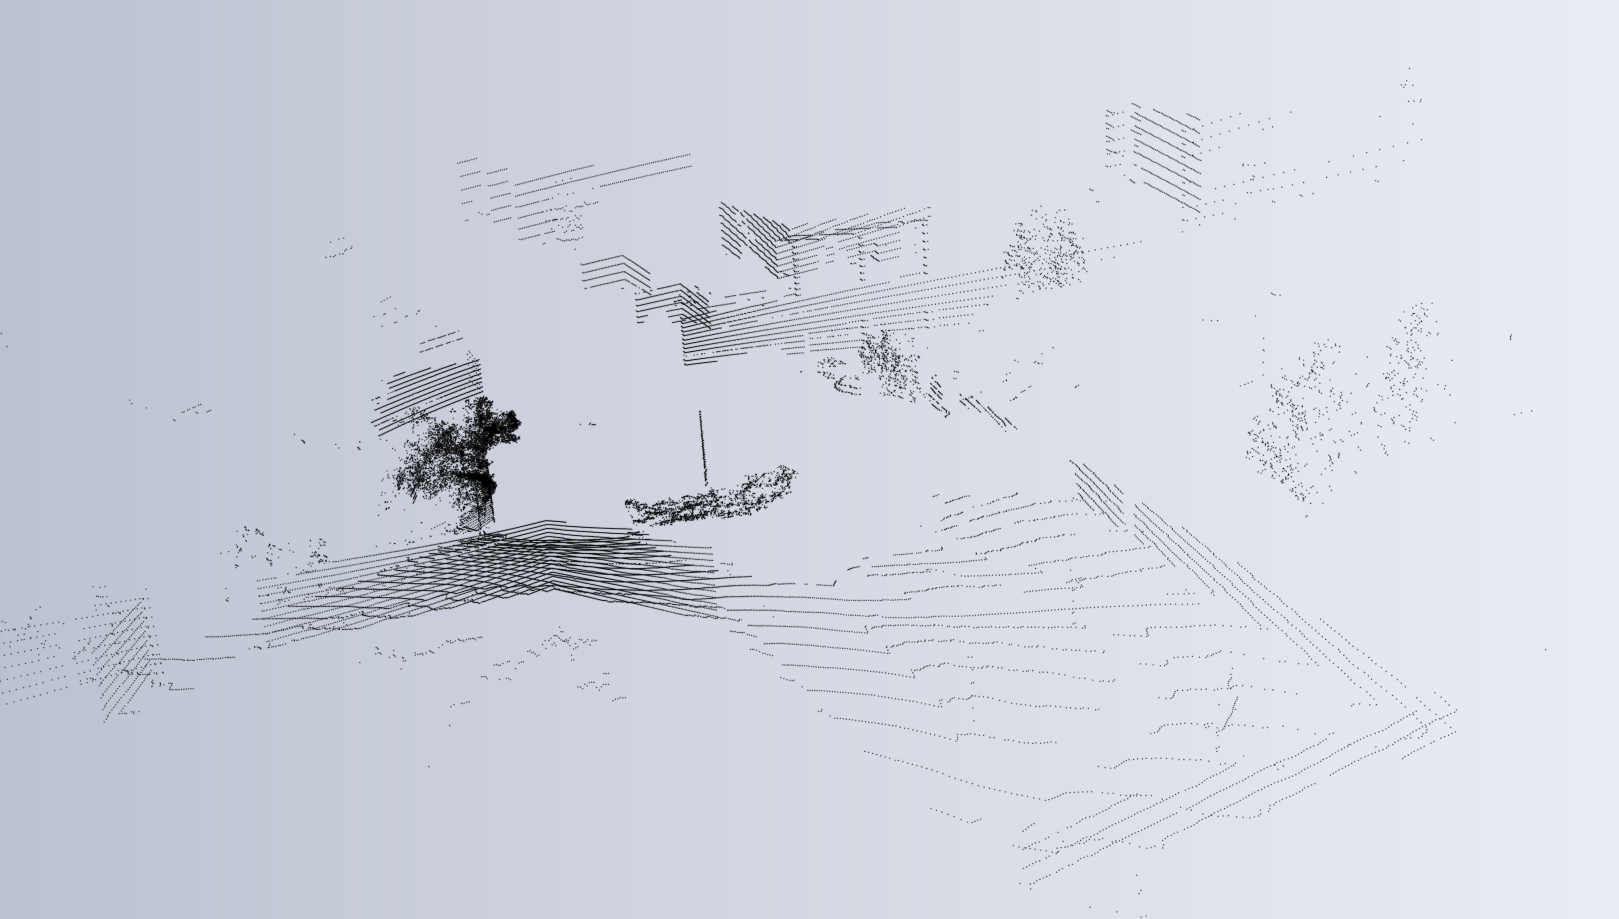
\includegraphics[width=\textwidth]{img_src/environement_lidar.png}
    \caption{Trame LIDAR}
    \label{fig:environnement_lidar}
\end{figure}

\vspace*{\fill}

\clearpage
\addtocontents{toc}{\protect\Needspace{15\baselineskip}}
\Needspace{12\baselineskip}
\section{Filtrage visuel intelligent par LoFTR et optimisation du recouvrement}

\hspace*{1cm}Cette troisième approche marquait un tournant dans la méthodologie de l'étude.\vspace{0.05cm}

\hspace*{1cm}Après avoir vérifié que le filtrage purement cinématique était utilisable pour la suppression des images statiques ou fortement redondantes, l'analyse a été poussée plus loin en s'intéressant au mécanisme interne du modèle \textbf{VGGT}. \vspace{0.1cm}

\hspace*{0.5cm}Le point crucial n'était pas uniquement la qualité visuelle des images, mais surtout leur \textbf{cohérence géométrique} entre elles.\vspace{0.2cm}

\hspace*{0.5cm}En effet, le modèle n'évaluait pas chaque vue de manière isolée : il dépendait fortement du \textbf{taux de recouvrement visuel} entre les différentes images pour établir des correspondances et estimer la cohérence de la scène ainsi que la stabilité de la calibration.\\

\par\bigskip
\par\bigskip

\subsection{Développement d'un module de sélection visuelle}

\hspace*{1cm}Au cours des premiers tests, il est apparu que l'envoi brut de séquences d'images conduisait à une surabondance d'informations. \vspace{0.1cm}

\hspace*{0.5cm}Lorsque le recouvrement entre deux vues était trop élevé, les images devenaient fortement redondantes et le modèle consommait inutilement des ressources de calcul sans apporter de gain géométrique significatif. \vspace{0.5cm}

\hspace*{1cm}À l'inverse, lorsque ce recouvrement était trop faible, les vues ne partageaient pas suffisamment d'informations communes pour permettre une estimation fiable de la pose relative et de l'auto-calibration extrinsèque. \vspace{0.1cm}

\hspace*{0.5cm}Cette observation a montré que le véritable problème ne résidait pas dans la quantité absolue d'images, mais davantage dans le \textbf{niveau de redondance géométrique} entre elles.\\


\hspace*{.5cm}Le cadre de mon stage était de participer à la conception d'un module de sélection visuelle capable de récupérer une séquence d'images. Son taux de recouvrement pouvait être contrôlé et modulé.\vspace{0.1cm}

\hspace*{.5cm}L'objectif était de ne conserver que les vues présentant un niveau de chevauchement spatial adapté au modèle, ni trop élevé, ni trop faible. Ce mécanisme devait ainsi permettre de réduire le nombre d'images transmises à VGGT sans dégrader la qualité de l'information géométrique utile à l'estimation.\\

\newpage

\subsection{Conditionnement et normalisation qualitative des images}

\hspace*{1cm}Avant toute mesure de recouvrement, les images était obligatoirement être préparées de manière homogène afin de ne pas introduire de biais artificiels dans l'évaluation. \vspace{0.05cm}

\hspace*{0.3cm}Pour cela, chaque trame a d'abord  été soumise à un pré-traitement visuel sous OpenCV.\\
Cette étape reposait principalement sur deux opérations : \vspace{0.2cm}

\begin{itemize}[itemsep=0.5em]

    \item \textbf{Correction de la distorsion optique :}\\
    \hspace*{0.5cm}Les paramètres intrinsèques fournis par le topic ROS~2 \texttt{camera\_info} étaient utilisés afin de corriger les effets de distorsion géométrique, notamment sur les caméras grand angle ou de type \textit{fisheye}. Cette correction devait permettre d'obtenir des images géométriquement cohérentes avant l'étape d'appariement.

    \vspace{0.5cm}

    \item \textbf{Filtrage photométrique des images saturées :}\\
    \hspace*{0.5cm}Les trames présentant une forte surexposition ou un éclairage défavorable étaient rejetées afin de garantir des conditions suffisamment robustes pour l'extraction et l'appariement des points caractéristiques.

\end{itemize}

\vspace{1cm}

\hspace*{1cm}Pour contourner cette limitation technique, un pipeline de découpage dynamique a été mis en place.\vspace{0.05cm}

\hspace*{0.5cm}Les séquences synchronisées extraites de chaque \texttt{rosbag} ont été partitionnées en blocs discrets de 20 images, appelés \textit{chunks}.\vspace{0.2cm}

\hspace*{1cm}Chaque bloc contenait des vues géométriquement cohérentes, tandis que les sorties du modèle, notamment les poses extrinsèques, les cartes de profondeur et les informations de scène, étaient sauvegardées sous forme de fichiers binaires compressés au format \texttt{.npy}.\\

\hspace*{1cm}Une nomenclature standardisée de type \texttt{predictions\_chunk\_XXXX.npy} a été utilisée afin d'identifier les différents blocs et de faciliter leur traitement ultérieur.\\
Cette stratégie devait limiter la consommation de mémoire GPU et d'assurer une exploitation progressive des résultats, tout en conservant une continuité suffisante entre les différentes portions de la séquence.

\clearpage

\subsection{Algorithme de concaténation et reconstruction de trajectoire}

\vspace{1cm}

\hspace*{1cm}Le traitement bloc par bloc ne suffisait pas, à lui seul, à reconstituer une trajectoire directement exploitable. Il était donc nécessaire de réassembler les résultats partiels dans un cadre spatio-temporel commun.\vspace{0.2cm}

\hspace*{1cm}Un algorithme de concaténation a été développé afin de fusionner les sorties obtenues sur chaque \textit{chunk}. Le principe reposait sur une fenêtre de recouvrement inter-blocs fixée à \textsb{n\_overlap = 3}.\\

\vspace{0.1cm}

\textsb{\hspace*{1cm}Cette étape de normalisation était essentielle, car un recouvrement calculé sur des images fortement bruitées, saturées ou déformées ne devenait pas nécessairement représentatif de la cohérence géométrique réelle entre les différentes vues.}

\vspace{1cm}

\subsection{Appariement dense par Transformer (LoFTR) et estimation du recouvrement}

\vspace{1cm}

\hspace*{1cm}Pour quantifier précisément le chevauchement entre deux images, le modèle de \textsb{\textit{deep learning}} \textbf{LoFTR} (\textsb{\textit{Local Feature Transformer}}) a été utilisé. \vspace{0.05cm}

\hspace*{0.5cm}Les méthodes traditionnelles sont basées sur des détecteurs locaux tels que \textsb{SIFT} ou \textsb{ORB}.\\
\hspace*{0.5cm}\textbf{LoFTR} repose sur une approche \textsb{\textit{detector-free}} permettant de réaliser un appariement dense de points d'intérêt à partir d'un mécanisme d'attention de type Transformer.\vspace{0.05cm}

\hspace*{1cm}Cette propriété était particulièrement adaptée à notre cas, car les scènes observées pouvaient présenter des zones faiblement texturées, des variations de luminosité ou encore des changements de perspective trés importants.\\

\hspace*{1cm}L'idée principielle a consisté dans la comparaison de deux images rectifiées \textsb{$I_{\text{ref}}$} et \textsb{$I_{\text{cand}}$}, puis à estimer le nombre et la distribution des correspondances géométriques entre celles-ci.\vspace{0.1cm}

\hspace*{1cm}À partir de cette densité de points homologues, il devenait possible de calculer un \textsb{taux de recouvrement visuel} exprimé en pourcentage. \vspace{0.05cm}

\hspace*{0.5cm}Cette mesure constituait alors un indicateur de la quantité d'informations commune entre les deux vues et permettait d'évaluer leur pertinence pour l'étape d'auto-calibration.

\newpage

\subsection{Développement des algorithmes de sélection sous consigne}

\hspace*{1cm}À partir de cette mesure de recouvrement, deux outils logiciels ont été développés en Python afin de sélectionner automatiquement les images les plus pertinentes :\vspace{0.2cm}
\begin{enumerate}[label=$\bullet$, itemsep=0.5em]

    \item \textbf{Génération de séquences panoramiques contrôlées :}\vspace{0.05cm}

    \hspace*{1cm}Le premier script parcourait les images de manière chronologique et conservait uniquement celles dont le taux de recouvrement visuel par rapport à la dernière image validée satisfaisait une consigne donnée.\vspace{0.05cm}

    \hspace*{1cm}Par exemple, une \textbf{valeur cible de $60\%$} permettait de maintenir une redondance géométrique suffisante tout en évitant de saturer inutilement l'ensemble de données.

\vspace{0.5cm}

    \item \textbf{Recherche itérative par consigne cible :}\vspace{0.05cm}

    \hspace*{1cm}Le second module effectuait une recherche globale sur l'ensemble du jeu de données. À partir d'une image de référence et d'une consigne définie par l'utilisateur, il évaluait les candidats disponibles, calculait leur recouvrement visuel à l'aide de LoFTR et sélectionnait l'image dont la valeur était la plus proche de la consigne cible.

\end{enumerate}

\par\bigskip
\par\bigskip

\subsection{Intérêt du contrôle du recouvrement pour le modèle VGGT}

\vspace{0.5cm}

\hspace*{1cm}L'originalité de cette approche a résidé dans le fait que la sélection des images n'était plus arbitraire, mais guidée par une contrainte géométrique explicite.\vspace{0.05cm}

\hspace*{0.3cm}Ainsi, au lieu de transmettre à VGGT une suite d'images très dense et potentiellement redondantes, l'objectif était de lui fournir une séquence plus compacte, plus informative et mieux adaptée à sa structure de traitement.\\

\hspace*{1cm}Cette optimisation devait permettre de réduire la quantité de données traitées et, par conséquent, la charge de calcul associée à l'inférence du modèle. Elle devait également favoriser la stabilité des estimations de pose et d'auto-calibration lorsque les images présentaient un niveau de recouvrement suffisamment cohérent.\vspace{0.05cm}

\hspace*{1cm}Ce formalisme pouvait ainsi alimenter le réseau avec des paires de vues présentant des caractéristiques géométriques contrôlées, ouvrant la voie à une analyse plus systématique de la sensibilité de VGGT face à différentes valeurs de recouvrement visuel.

\newpage


\section{Mise en place et suivi des solutions}

\vspace{1cm}

\hspace*{1cm}La mise en place des solutions développées a constitué la phase de transition entre le constat théorique et l'évaluation expérimentale.\vspace{0.3cm}

\hspace*{1cm}L'objectif n'était pas seulement de corriger les défauts liés à la qualité des données, mais de construire un pipeline complet, cohérent et exploitable sur des séquences réelles de navigation autonome.\vspace{0.1cm}

\hspace*{1cm}Cette étape a permis de passer d'une observation qualitative des problèmes rencontrés, notamment la redondance, la dérive, les défauts de synchronisation ou encore le recouvrement insuffisant, à une mise en œuvre concrète, pilotée par des règles géométriques et des contraintes de calcul.

\vspace{2cm}

\subsection{Filtrage cinématique (Arrêt du véhicule)}

\vspace{1cm}

\hspace*{1cm}Le filtrage cinématique a constitué la première couche du traitement mis en place afin d'isoler les images pertinentes et d'éliminer les trames non exploitables pour l'analyse géométrique.\\

\hspace*{1cm}Son rôle principal était de supprimer les phases de déplacements parasites, les phénomènes de bougé ainsi que les instants durant lesquels le véhicule ne se trouvait pas dans une configuration suffisamment stable pour la calibration.\vspace{0.05cm}

\hspace*{1cm}Cette opération a permis d'obtenir des séquences plus nettes, plus homogènes et mieux adaptées à l'analyse par le modèle \textbf{VGGT}.

\newpage

\subsection{Architecture d'extraction et traitement par blocs (\textit{Chunks})}

\hspace*{1cm}Compte tenu de la complexité structurelle du réseau \textbf{VGGT}, l'inférence directe sur de longues séquences vidéo s'est révélée inadaptée aux contraintes de mémoire GPU et de temps de calcul.\\

\hspace*{1cm}Pour contourner cette limitation technique, un pipeline de découpage dynamique a été mis en place. Les séquences synchronisées extraites de chaque \texttt{rosbag} ont été partitionnées en blocs discrets de 20 images, appelés \textit{chunks}.\vspace{0.05cm}

\hspace*{1cm}Chaque bloc contenait des vues géométriquement cohérentes, tandis que les sorties du modèle, notamment les poses extrinsèques, les cartes de profondeur et les informations de scène, étaient sauvegardées sous forme de fichiers binaires compressés au format \texttt{.npy}.\\

\hspace*{1cm}Une nomenclature standardisée de type \texttt{predictions\_chunk\_XXXX.npy} a été utilisée afin d'identifier les différents blocs et de faciliter leur traitement ultérieur.\vspace{0.05cm}

\hspace*{.5cm}Cette stratégie a permis de limiter la consommation de mémoire GPU et d'assurer une exploitation progressive des résultats, tout en conservant une continuité suffisante entre les différentes portions de la séquence.

\vspace{0.cm}

\subsection{Algorithme de concaténation et reconstruction de trajectoire}

\hspace*{1cm}Le traitement bloc par bloc ne suffisant pas, à lui seul, à reconstituer une trajectoire directement exploitable.\vspace{0.05cm}

\textbf{\hspace*{1cm}Il était donc nécessaire de réassembler les résultats partiels dans un cadre spatio-temporel commun.\vspace{0.1cm}}

\hspace*{1cm}Un algorithme de concaténation a donc été développé afin de fusionner les sorties obtenues sur chaque \textit{chunk}.\vspace{0.05cm}

\hspace{1cm}Le principe reposait sur une fenêtre de recouvrement inter-blocs fixée à : \\ 
\vspace{0.03cm}
\noindent\makebox[\textwidth][c]{\textsb{n\_overlap = 3}}

\vspace{0.2cm}

\hspace*{1cm}Cette zone commune permettait d'estimer les transformations homogènes nécessaires pour relier un bloc à son prédécesseur.\vspace{0.05cm}

\hspace*{.5cm}En exploitant ensuite les vecteurs de translation associés aux différentes poses des caméras réalignées, il devenait possible de reconstruire progressivement une trajectoire continue du véhicule sur l'ensemble de la séquence.

\newpage

\subsection{Stratégies de recalage face à la vérité terrain (GPS)}

\hspace*{1cm}La trajectoire reconstruite par \textbf{VGGT} n'était pas directement comparable à la référence géométrique, car elle était exprimée dans un référentiel relatif et pouvait être affectée par une dérive au cours du temps.\vspace{0.2cm}

\hspace*{1cm}Pour résoudre cette problèmatique, les données GPS enregistrées en parallèle ont été utilisées comme références de positionnement. \vspace{0.05cm}

\hspace*{0.5cm}L'alignement des trajectoires devait s'effectué en deux étapes successives :\vspace{0.05cm}

\begin{enumerate}[label=$\bullet$, itemsep=1em]

    \item \textbf{Recalage global par similitude 2D ($\text{Sim}(2)$) :}\vspace{0.05cm}

    \hspace*{1cm}Une première transformation globale devait aligner les trajectoires dans un même espace métrique. \\
    \hspace*{0.5cm}Elle combinait un angle de rotation $\theta$, un facteur d'échelle $s$ ainsi qu'un \textsb{vecteur de translation $t = [t_x, t_y]^T$}.\vspace{0.05cm}

    \hspace*{.5cm}L'optimisation a été réalisée à l'aide d'un estimateur robuste basé sur la fonction de \textbf{coût de Huber} afin de limiter l'influence des éventuels points aberrants présents dans les données.

    \item \textbf{Recalage hiérarchique récursif (\textit{Piecewise split}) :}\vspace{0.05cm}

    \hspace*{1cm}Après l'alignement global, des écarts locaux persistants pouvaient être observés sur certaines portions de la trajectoire. Afin de corriger ces déformations non uniformes, un recalage récursif était appliqué.\vspace{0.05cm}

    \hspace*{0.5cm}Lorsque l'écart local entre la trajectoire estimée par \textbf{VGGT} et la référence GPS dépassait un seuil défini, le segment concerné était découpé et une nouvelle transformation locale était estimée sur cette portion.

\end{enumerate}

\vspace{1cm}

\hspace*{0.5cm}\textsb{Cette stratégie devait permettre :} \vspace{0.05cm}

\begin{itemize}[label=\textbullet, itemsep=0.5em, leftmargin=2cm]
    \item \textsb{Un meilleur compte rendu des erreurs locales liées à la dérive visuelle}

    \item \textsb{De conserver une cohérence globale de la trajectoire reconstruite}

\end{itemize}

\vspace{0.2cm}

\hspace*{0.5cm}\textsb{Toutefois, elle n'a pas pu être pleinement exploitée, car les résultats obtenus de la reconstruction de VGGT n'ont pas permis d'établir une comparaison visuelle suffisamment claire et pertinente.}

\newpage

\subsection{Suivi du filtrage intelligent par LoFTR}

\vspace{1cm}

\hspace*{1cm}En parallèle, le module de sélection visuelle basé sur \textbf{LoFTR} a été intégré en amont du traitement par blocs. \vspace{0.01cm}

\hspace*{0.5cm}Sa fonction consistait à réguler la densité géométrique des vues transmises au modèle en évaluant leur niveau de recouvrement visuel.\vspace{0.1cm}

\hspace*{1cm}Les trames présentant un recouvrement trop important, \textbf{supérieur à $80\%$}, ou fortement influencées par un mouvement parasite étaient éliminées. \vspace{0.01cm}

\hspace*{0.5cm}Cette sélection organisait l'\textbf{optimiser la répartition des 20 images de chaque bloc} vers des zones présentant une valeur ajoutée géométrique plus importante.\vspace{0.1cm}

\hspace*{1cm}L'objectif était ainsi d'éviter de saturer inutilement le réseau avec des vues fortement redondantes, tout en conservant suffisamment d'informations communes entre les différentes images pour permettre une estimation géométrique cohérente.\vspace{1.5cm}

\hspace*{1cm}\textsb{Dans l'ensemble, cette première couche de mise en œuvre a montré que la qualité de la calibration dépendait autant du modèle utilisé que de la manière dont les données étaient filtrées, ordonnées et réassemblées.}

\newpage

\section{Bilan}

\vspace{1.6cm}


\hspace*{1cm}L'évaluation du pipeline de traitement a permis de dresser un bilan global, à la fois quantitatif et qualitatif. \vspace{0.5cm}

\hspace*{0.5cm}Il apparaît clairement que la \textbf{qualité des résultats} ne dépend pas uniquement du modèle d'IA utilisé, mais également de la \textbf{cohérence} et de la \textbf{richesse géométrique} des données qui lui sont transmises.\vspace{0.1cm}

\hspace*{1cm}La première approche explorée au début du stage n'a pas permis d'aboutir à une reconstruction suffisamment satisfaisante.\vspace{0.03cm}

\hspace*{0.5cm} La stabilisation des résultats n'a été observée qu'avec la méthode de filtrage visuel intelligent basée sur \textbf{LoFTR}, qui a permis de sélectionner les vues les plus pertinentes et d'optimiser le recouvrement géométrique entre images. \vspace{0.5cm}

\vspace{1cm}

\noindent\textbf{\uline{\large Cette méthode c'est-elle révélée être le point de bascule du projet ?}}\par
\medskip

\vspace{0.5cm}

\hspace*{1cm}Elle a induit une gestion des données plus cohérente et une reconstruction effectivement exploitable.\vspace{0.03cm}

\hspace*{0.5cm}La réalisation d'une réalité terrain plus fiable à partir des données LiDAR et SLAM, a permis de \textbf{valider cette approche dans un cadre plus rigoureux}.\vspace{0.6cm}

\hspace*{1cm}La synchronisation de filtrage cinématique et de génération d'une vérité terrain à partir des données LiDAR/SLAM ont permis de renforcer cette approche, en réduisant les redondances, les zones de faible valeur informative ainsi que les distorsions temporelles.\vspace{0.2cm}

\hspace*{1cm}Le bilan repose donc sur un constat général :\vspace{0.01cm}

\begin{itemize}[label=\textbullet, itemsep=0.5em, leftmargin=2cm]

    \item \textbf{Le pré-traitement des données constitue une étape fondamentale du processus d'estimation}

\end{itemize}

\vspace{0.3cm}

\hspace*{0.5cm}\textsb{Il ne peut être considéré comme un simple accessoire d'optimisation}


\newpage

\noindent\textbf{\uline{\large Que révèlent les analyses quantitatives des résultats de reconstruction ?}}\par
\medskip

\vspace{1cm}

\hspace*{1cm}L'installation d'un recalage hiérarchique par morceaux (\textit{piecewise}) s'est avérée essentielle pour corriger les déformations locales de la trajectoire autour du rond-point.\vspace{0.01cm}

\hspace*{1cm}Après une étape de rééchantillonnage linéaire, l'estimation de la trajectoire a pu être confrontée à la vérité terrain GPS avec une cohérence acceptable sur l'ensemble du parcours.\\
\hspace*{.5cm}Cette comparaison a permis de vérifier la capacité du modèle à restituer la structure globale de la trajectoire malgré les erreurs accumulées au cours de la séquence.\vspace{0.1cm}

\hspace*{1cm}Ces résultats nous ont indiqué que le modèle était capable de restituer la structure globale de la trajectoire, mais qu'il restait sensible aux zones présentant une forte dynamique angulaire ainsi qu'aux variations locales du recouvrement visuel.\vspace{0.05cm}

\hspace*{1cm}La reconstruction globale pouvait être ainsi considérée comme cohérente, tandis que l'estimation locale demeurait plus imparfaite et nécessitait l'introduction de contraintes géométriques supplémentaires pour améliorer sa précision.

\vspace{1cm}

\noindent\textbf{\uline{\large Dans quelles mesure les limites techniques et les biais impactent les résultats ?}}\par
\medskip

\vspace{0.5cm}

\hspace*{1cm}L'analyse critique des écarts résiduels ont mis en évidence plusieurs facteurs limitants susceptibles d'affecter la précision finale du pipeline. \\
\hspace*{0.5cm}Trois limitations principales ont été identifiées :\vspace{0.02cm}

\begin{enumerate}[itemsep=0.5em]

    \item{\textbf{Dérive cumulative monoculaire :}}\vspace{0.02cm}

    \hspace*{1cm}Le modèle \textbf{VGGT} reste soumis aux limitations intrinsèques des approches reposant principalement sur l'information visuelle. \vspace{0.01cm}

    \hspace*{0.5cm}Des erreurs de pose faibles mais persistantes pouvaient s'accumuler au fil des vues et entraîner progressivement des déformations géométriques de la trajectoire reconstruite.\vspace{0.03cm}

    \hspace*{1cm}L'élimination total de cette dérive ne pouvait être envisagée qu'avec l'introduction d'un traitement global supplémentaire, par exemple :\vspace{0.05cm}

    \begin{itemize}[label=\textbullet, leftmargin=2cm, itemsep=0.5em]
        \item \textbf{Introduction d'une boucle de fermeture (\textit{loop closure})}
        \item \textbf{Optimisation globale de type ajustement de faisceaux (\textit{bundle adjustment})}
    \end{itemize}

\newpage

    \item{\textbf{Désynchronisation temporelle et biais d'interpolation :}}\vspace{0.02cm}

    \hspace*{1cm}La comparaison directe entre des trajectoires issues de capteurs hétérogènes est naturellement soumise à des décalages temporels.\vspace{0.05cm}

    \hspace*{0.5cm}L'interpolation linéaire utilisée pour aligner les différentes séries temporelles permet de réduire ce biais, mais ne suffit pas nécessairement à le supprimer totalement, notamment lors des phases d'accélération, de freinage ou de changement de direction.

    \item{\textbf{Sensibilité aux conditions visuelles :}}\vspace{0.02cm}

    \hspace*{1cm}Les images acquises dans des conditions de luminosisté variables ou présentant une forte distorsion optique peuvent conduire à des appariements visuels moins fiables.\vspace{0.05cm}

    \hspace*{0.5cm}Cette dégradation affecte directement la sélection géométrique des vues par \textbf{LoFTR} et peut, par conséquent, influencer la qualité des estimations produites lors de l'étape d'auto-calibration.

\end{enumerate}

\vspace{1cm}

\noindent\textbf{\uline{\large Vers une auto-calibration extrinsèque : quelles voies d'évolution ?}}\par
\medskip

\vspace{0.5cm}

\hspace*{1cm}Malgré ces limitations, les travaux ont confirmeé la pertinence d'une stratégie reposant sur le conditionnement préalable des données. \vspace{0.1cm}

\hspace*{0.5cm}L'objectif à terme est de coupler de manière plus systématique les séquences visuelles filtrées selon un recouvrement optimal avec une vérité terrain générée à partir du \textbf{Kitware LiDAR SLAM}.\vspace{0.1cm}

\hspace*{1cm}Dans cette perspective, les images ont été d'abord corrigées de leur distorsion intrinsèque, puis projetées dans un repère virtuel défini par le LiDAR afin d'établir une correspondance géométrique entre les observations visuelles et la reconstruction tridimensionnelle.\vspace{0.5cm}

\hspace*{1cm}Cette approche a permis d'isoler plus précisément les paramètres associés à l'auto-calibration extrinsèque des différentes caméras. \vspace{0.05cm}

\hspace*{0.5cm}Le protocole envisagé pouvait ainsi permettre de mesurer, dans des conditions contrôlées et indépendamment de la dynamique du véhicule, la précision métrique de l'orientation relative entre les différents capteurs.\vspace{0.1cm}

\hspace*{0.5cm}Une telle référence fournirait également un cadre de comparaison plus rigoureux pour les travaux futurs, notamment pour quantifier les améliorations apportées par les différentes stratégies de filtrage et de sélection des images.

\newpage

\vspace{1cm}

\hspace*{1cm}\textbf{Pour cette étude, VGGT n'a pas répondu aux attentes définies au départ.}\vspace{0.05cm}

\hspace*{1cm}\textbf{Mais elle a confirme la faisabilité d'un pipeline de traitement adapté aux données réelles issues d'un véhicule autonome.}\vspace{1cm}

\hspace*{1cm}Les résultats obtenus n'étaient pas encore suffisants pour atteindre une précision de calibration millimétrique entièrement automatique. \vspace{0.01cm}

\hspace*{0.5cm}Ils démontraient néanmoins que l'optimisation du filtrage, la synchronisation des données et la structuration géométrique des entrées du modèle constituent des leviers majeurs pour améliorer la robustesse et la qualité des estimations.\vspace{0.5cm}

\hspace*{1cm}Le travail réalisé a fournit ainsi une base méthodologique pour poursuivre l'étude de l'auto-calibration extrinsèque en combinant de manière plus étroite les informations visuelles issues de \textbf{VGGT}, les correspondances géométriques obtenues avec \textbf{LoFTR} et la référence tridimensionnelle fournie par le LiDAR.

% ==============================================================================
% CONCLUSION, BIBLIO & ANNEXES
% ==============================================================================

\chapter*{Conclusion}
\addcontentsline{toc}{chapter}{Conclusion}

\hspace*{1cm}Ce stage a permis d'aborder un enjeu central de la robotique autonome : la qualité de la perception ne dépend pas uniquement des capteurs utilisés, mais également de la manière dont les données sont préparées, synchronisées et exploitées.\\
À travers l'étude du modèle \textbf{VGGT} et des données issues de la plateforme \textbf{PAVIN}, un constat fondamental a pu être mis en évidence : l'utilisation directe de séquences vidéo présentant une forte redondance n'est pas nécessairement adaptée à un modèle de géométrie visuelle particulièrement coûteux en ressources de calcul.\\

\hspace*{1cm}Le prétraitement des données apparaît ainsi comme une étape nécessaire, voire déterminante, pour améliorer la stabilité des estimations, limiter la dérive de reconstruction et exploiter plus efficacement les capacités du modèle.

\par\bigskip
\par\bigskip

\hspace*{0.4cm}\textbf{Apports scientifiques}\\

\hspace*{.3cm}Les travaux réalisés au cours de ce stage ont permis de développer et d'évaluer plusieurs briques de traitement destinées à améliorer la qualité des données fournies au modèle. Les principaux apports scientifiques peuvent être résumés de la manière suivante :

\begin{itemize}[itemsep=0.5em]
    \item Développement d'un pipeline de synchronisation temporelle et de filtrage de flux de données hétérogènes ;
    
    \item Étude du comportement du modèle \textbf{VGGT} face à des données réelles issues d'une plateforme robotique autonome et analyse de l'influence de la redondance géométrique ;
    
    \item Mise en place d'un module de sélection d'images fondé sur l'analyse du recouvrement visuel à l'aide de \textbf{LoFTR} ;
    
    \item Développement d'une stratégie de comparaison avec une vérité terrain obtenue à partir des données LiDAR et des trajectoires issues du SLAM ;
    
    \item Mise en évidence de l'influence du conditionnement des données sur la qualité des estimations de pose et sur la stabilité de la reconstruction géométrique.
\end{itemize}

\par\bigskip
\par\bigskip

\hspace*{0.4cm}\textbf{Apports professionnels}\\

\hspace*{.3cm}Au-delà des résultats scientifiques obtenus, ce stage m'a également permis de développer plusieurs compétences techniques et méthodologiques directement liées aux problématiques de perception robotique et de recherche expérimentale :

\begin{itemize}[itemsep=0.5em]
    \item Acquisition de compétences avancées en perception multi-capteurs et en robotique autonome ;
    
    \item Maîtrise d'outils de développement scientifique et robotique tels que \textbf{ROS~2}, \textbf{Python}, \textbf{OpenCV} ainsi que des méthodes de traitement de nuages de points ;
    
    \item Développement de compétences en analyse de données, en conception d'algorithmes de filtrage et en évaluation expérimentale ;
    
    \item Acquisition d'une expérience dans la mise en œuvre d'un pipeline complet, depuis l'extraction des données issues du \texttt{rosbag} jusqu'à leur exploitation pour l'analyse géométrique ;
    
    \item Développement d'une capacité à formaliser un problème technique, à identifier ses limitations et à proposer une solution structurée pouvant être évaluée expérimentalement.
\end{itemize}

\par\bigskip
\par\bigskip

\hspace*{0.4cm}\textbf{Perspectives}\\

\hspace*{.3cm}Les résultats obtenus au cours de ce stage ouvrent plusieurs perspectives de poursuite. La prochaine étape consiste à coupler de manière plus systématique les séquences visuelles sélectionnées selon un recouvrement géométrique optimal avec la vérité terrain générée à partir des données LiDAR et du SLAM.\\
Cette association permettrait de quantifier plus rigoureusement la précision de l'auto-calibration extrinsèque des différentes caméras et d'établir une comparaison métrique entre les estimations produites par \textbf{VGGT} et une référence tridimensionnelle indépendante.\\

\hspace*{.3cm}L'amélioration du conditionnement des images constitue également une perspective importante. La correction systématique de la distorsion optique ainsi qu'une meilleure gestion des variations de luminosité pourraient contribuer à renforcer la robustesse des correspondances visuelles et, par conséquent, la stabilité de l'estimation géométrique.\\
\hspace*{.5cm}Enfin, les méthodes développées pourraient être évaluées sur des scénarios plus variés, notamment dans des environnements urbains plus complexes, sur des trajectoires plus longues ou dans des conditions de déplacement différentes. Cette extension permettrait d'étudier la capacité de généralisation du pipeline et d'identifier les limites de son fonctionnement dans des situations plus représentatives d'une utilisation opérationnelle.

\par\bigskip

\hspace*{.3cm}En somme, ce stage a permis de mettre en évidence l'importance du prétraitement et du conditionnement des données dans les systèmes modernes de perception robotique.\\

\hspace*{.3cm}Les expérimentations réalisées montrent que des performances robustes en reconstruction géométrique et en calibration ne dépendent pas uniquement de l'architecture du modèle utilisé, mais également de la qualité, de la cohérence temporelle et de la pertinence géométrique des informations qui lui sont transmises.\\
\hspace*{.3cm}La combinaison du filtrage cinématique, de la sélection visuelle par \textbf{LoFTR}, de l'exploitation des données LiDAR et de la comparaison avec une référence SLAM constitue ainsi une approche cohérente pour améliorer l'exploitation de modèles de géométrie visuelle tels que \textbf{VGGT}.\\

\hspace*{.3cm}Cette démarche constitue une base solide pour la poursuite des travaux du laboratoire sur l'auto-calibration multi-capteurs et, plus largement, pour le développement de systèmes de perception autonomes plus fiables, plus robustes et mieux adaptés aux contraintes des plateformes robotiques réelles.


% ==============================================================================
% BIBLIOGRAPHIE ET RÉFÉRENCES
% ==============================================================================
\begin{thebibliography}{99}
\addcontentsline{toc}{chapter}{Bibliographie}

\bibitem{institut_pascal_site}
Institut Pascal, \textit{Site officiel de l'Institut Pascal - Présentation et activités}, Université Clermont Auvergne, 2024. URL: \url{https://www.institut-pascal.fr/}.

\bibitem{uca_institut_pascal}
Université Clermont Auvergne, \textit{Présentation de l'Institut Pascal (IP)}, Annuaire des laboratoires UCA, 2026. URL: \url{https://www.uca.fr/laboratoires/institut-pascal-ip}.

\bibitem{slam_survey}
J. Zhang et S. Singh, \textit{``A Survey on Visual Odometry and Visual SLAM''}, IEEE Transactions on Robotics, vol. 38, no. 2, pp. 367-391, mars 2022.

\bibitem{sensor_fusion}
R. Mur-Artal et J. M. M. Montiel, \textit{``Multi-Sensor Fusion for Robust SLAM in Dynamic Environments''}, IEEE International Conference on Robotics and Automation (ICRA), Paris, France, pp. 1234-1240, mai 2023.

\bibitem{ros2_docs}
Open Robotics, \textit{ROS 2 Documentation: Design and Architecture}, Open Robotics, 2024. URL: \url{https://docs.ros.org/en/humble/}.

\bibitem{pavine_platform}
CNRS, \textit{PAVIN - Plateforme Auvergnate Pour les Véhicules Intelligents}, CNRS, 2023. URL: \url{https://www.pavin.fr/}.

\bibitem{vggt_repo}
Facebook Research, \textit{VGGT: Visual Geometry Grounded Transformer}, GitHub repository, 2024. URL: \url{https://github.com/facebookresearch/vggt}.

\bibitem{vggt_paper}
M. Wang, J. Ren, J. Li, Y. Zhu, F. Yang et al., \textit{``VGGT: Visual Geometry Grounded Transformer''}, arXiv preprint, 2025. URL: \url{https://arxiv.org/}.

\bibitem{loftr_paper}
J. Sun, Z. Shen, Y. Wang, H. Bao et al., \textit{``LoFTR: Detector-Free Local Feature Matching with Transformers''}, IEEE Conference on Computer Vision and Pattern Recognition (CVPR), 2021.

\bibitem{lidar_slam_survey}
C. Cadena, L. Carlone, H. Carrillo, Y. Latif, D. Scaramuzza et al., \textit{``Past, Present, and Future of Simultaneous Localization and Mapping: Toward the Robust-Perception Age''}, IEEE Transactions on Robotics, vol. 32, no. 6, pp. 1309-1332, 2016.

\bibitem{multisensor_fusion}
A. Censi, \textit{``On Sensor Fusion and Calibration in Robotics''}, International Journal of Robotics Research, 2019.

\end{thebibliography}

\newpage

% ==============================================================================
% TABLE DES ILLUSTRATIONS
% ==============================================================================

\listoffigures
\cleardoublepage

% ==============================================================================
% ANNEXES
% ==============================================================================
\appendix
\chapter*{Annexes}
\addcontentsline{toc}{chapter}{Annexes}
\printannextoc

\annexchapter{Compléments techniques sur VGGT}

\annexsection{Objectif et principe général}

VGGT (\textit{Visual Geometry Grounded Transformer}) est un modèle d'apprentissage profond conçu pour estimer la géométrie d'une scène à partir d'un ensemble d'images. Son objectif est de produire directement, en une seule passe d'inférence, plusieurs informations utiles à la reconstruction tridimensionnelle : les paramètres des caméras, les cartes de profondeur, les \textit{point maps} et le suivi de points entre les différentes vues.

Cette approche se distingue d'un pipeline classique de type Structure-from-Motion (SfM). Dans un pipeline SfM, les caractéristiques visuelles sont d'abord détectées, puis mises en correspondance entre les images. Les poses des caméras et la structure 3D sont ensuite estimées par triangulation avant d'être raffinées par ajustement de faisceaux. VGGT regroupe une grande partie de ces étapes dans un modèle feed-forward : les images sont fournies au réseau et les sorties géométriques sont prédites directement.

Le caractère feed-forward simplifie le traitement et permet de produire rapidement une première estimation. Toutefois, les sorties restent sensibles à la qualité des images, au recouvrement entre les vues, aux mouvements de la caméra et à la cohérence de la séquence fournie en entrée. Dans le cadre de ce stage, le pré-traitement des images constitue donc une étape indispensable avant l'inférence.

\annexsection{Représentation des images et des tokens}

Chaque image d'entrée est découpée en petites régions, appelées \textit{patches}. Ces régions sont transformées en représentations numériques appelées \textit{tokens visuels}. Cette représentation permet au Transformer de manipuler simultanément le contenu de l'image et les relations entre les différentes vues.

À ces tokens visuels sont associés des \textit{camera tokens}. Ils servent à concentrer l'information nécessaire à l'estimation des paramètres de caméra. Pour une séquence de $N$ images, le réseau construit ainsi une représentation combinant les informations propres à chaque image et les informations communes à l'ensemble de la séquence.

On peut représenter cette étape de manière simplifiée par :
\begin{equation}
    I_i \longrightarrow H_i = \{h_{i,1}, h_{i,2}, \ldots, h_{i,P}\},
\end{equation}
où $I_i$ désigne la $i$-ième image, $H_i$ sa représentation sous forme de tokens et $P$ le nombre de patches utilisés pour cette image.

\annexsection{Mécanisme d'attention alternée}

Le cœur de VGGT repose sur l'alternance de deux mécanismes d'attention complémentaires.

\annexsubsection{Attention au sein d'une image}

L'attention de type \textit{frame-wise} traite les tokens appartenant à une même image. Elle permet au réseau de consolider les relations spatiales locales, les contours, les textures et les éléments de structure visibles dans chaque vue. Cette étape contribue à construire une représentation cohérente de la scène observée par une caméra donnée.

\annexsubsection{Attention globale entre les vues}

L'attention globale met ensuite en relation les tokens provenant des différentes images. Le réseau peut ainsi comparer les observations, identifier les éléments communs et exploiter la parallaxe entre les vues. Cette information est essentielle pour estimer les relations géométriques entre les caméras et reconstruire une structure 3D cohérente.

L'alternance de ces deux attentions peut être résumée par :
\begin{equation}
    H^{(l+1)} = \mathcal{A}_{\mathrm{global}}
    \left(\mathcal{A}_{\mathrm{frame}}(H^{(l)})\right),
\end{equation}
où $H^{(l)}$ désigne les représentations internes à la couche $l$, tandis que $\mathcal{A}_{\mathrm{frame}}$ et $\mathcal{A}_{\mathrm{global}}$ représentent respectivement l'attention intra-image et l'attention inter-images.

\annexsection{Têtes de prédiction et sorties géométriques}

Après la fusion des informations par le Transformer, plusieurs têtes spécialisées produisent les sorties géométriques du modèle.

\annexsubsection{Paramètres et poses des caméras}

La \textit{camera head} exploite notamment les \textit{camera tokens} pour estimer les paramètres associés aux vues. Les paramètres intrinsèques décrivent les propriétés internes de la caméra, comme la focale et le centre principal. Les paramètres extrinsèques décrivent la position et l'orientation de la caméra dans un repère donné.

Une pose peut être représentée par une transformation rigide :
\begin{equation}
    \mathbf{T}_i =
    \begin{bmatrix}
        \mathbf{R}_i & \mathbf{t}_i \\
        \mathbf{0}^{\mathsf{T}} & 1
    \end{bmatrix},
\end{equation}
où $\mathbf{R}_i \in SO(3)$ est la matrice de rotation et $\mathbf{t}_i \in \mathbb{R}^3$ le vecteur de translation de la caméra $i$. Dans la pratique, les poses prédites par VGGT sont utilisées pour extraire une trajectoire relative. Cette trajectoire doit ensuite être alignée sur une référence métrique, comme une trajectoire GPS ou une trajectoire obtenue par LiDAR-SLAM.

\annexsubsection{Cartes de profondeur}

La tête dense du modèle produit une carte de profondeur pour chaque image. À chaque pixel est associée une estimation de sa distance par rapport à la caméra. Ces cartes permettent de représenter la structure de la scène sous une forme dense, contrairement au nuage de points clairsemé produit par les premières étapes d'un pipeline SfM classique.

La profondeur prédite ne doit cependant pas être considérée automatiquement comme une mesure métrique parfaite. Selon les conditions d'inférence, elle peut être affectée par une ambiguïté d'échelle, des surfaces peu texturées, des occultations ou des erreurs de prédiction locales.

\annexsubsection{Point maps}

Une \textit{point map} associe à chaque pixel une position 3D estimée. Elle peut être vue comme une représentation dense de la scène dans laquelle les pixels ne sont plus seulement décrits par leur intensité ou leur couleur, mais aussi par des coordonnées spatiales.

Cette sortie est particulièrement intéressante pour analyser la cohérence géométrique d'une reconstruction. Elle peut également servir à comparer les observations issues des différentes vues et à identifier les zones où la géométrie prédite est peu fiable.

\annexsubsection{Suivi de points entre les images}

VGGT fournit également des informations de suivi de points 3D à travers les vues. Le principe consiste à retrouver, dans plusieurs images, les projections correspondant à un même élément de la scène. Ces correspondances contribuent à maintenir une cohérence multi-vues et à relier les représentations produites pour chaque image.

\annexsection{Déroulement d'une inférence}

Dans l'application étudiée, le déroulement d'une inférence peut être décrit en plusieurs étapes :
\begin{enumerate}
    \item les images sont extraites de la vidéo ou du fichier de données ;
    \item les images sont triées et, si nécessaire, sous-échantillonnées afin de limiter la redondance ;
    \item un groupe d'images est chargé par le modèle, généralement sous la forme d'un bloc de taille limitée ;
    \item les images sont converties en tokens et traitées par les mécanismes d'attention ;
    \item les têtes de prédiction calculent les poses, les cartes de profondeur, les point maps et les informations de suivi ;
    \item les sorties sont sauvegardées afin d'être analysées ou utilisées lors de la reconstruction de trajectoire.
\end{enumerate}

Le traitement par blocs est nécessaire lorsque la séquence complète est trop volumineuse pour être traitée en une seule fois. Dans le rapport, les sorties de chaque bloc sont ensuite alignées et concaténées. Cette opération introduit toutefois un risque de discontinuité entre deux blocs, car chaque inférence peut produire un repère relatif ou une échelle différente.

\annexsection{Intérêt du pré-traitement pour VGGT}

Le fonctionnement de VGGT dépend fortement de la qualité du jeu d'images fourni. Des images trop proches dans le temps apportent une information redondante et augmentent le coût de calcul. À l'inverse, des images trop éloignées peuvent présenter un recouvrement insuffisant, ce qui complique l'établissement des relations géométriques.

Le filtrage cinématique permet d'éliminer certaines images prises pendant des phases peu utiles, par exemple lorsque le véhicule est immobile ou lorsque le flou de bougé dégrade fortement la qualité visuelle. La synchronisation garantit que les observations utilisées pour une même étape correspondent à des instants comparables. Enfin, la sélection fondée sur le recouvrement visuel permet de rechercher un compromis entre redondance et continuité géométrique.

Cette préparation ne modifie pas l'architecture de VGGT. Elle agit en amont, en contrôlant les données transmises au modèle afin de rendre l'inférence plus stable et plus exploitable dans un contexte de reconstruction de trajectoire.

\annexsection{Limites dans le contexte de l'étude}

Plusieurs limites doivent être prises en compte lors de l'interprétation des résultats :
\begin{itemize}
    \item les poses prédites à partir d'une caméra seule sont sujettes à une dérive cumulative lorsque les sorties sont concaténées sur une longue séquence ;
    \item l'échelle et l'orientation de la trajectoire doivent être recalées sur une référence externe pour permettre une comparaison métrique ;
    \item les changements rapides de direction, les zones peu texturées et les variations d'éclairage peuvent dégrader la qualité des sorties ;
    \item un décalage temporel entre les images et la référence GPS ou LiDAR peut produire une erreur lors de la comparaison point à point ;
    \item le traitement par blocs limite la mémoire nécessaire, mais rend nécessaire une étape supplémentaire d'alignement entre les segments.
\end{itemize}

Ainsi, VGGT doit être considéré comme un estimateur géométrique puissant fournissant une reconstruction initiale, et non comme une solution complète de calibration métrique indépendante de toute référence. Dans le cadre de ce stage, son intérêt réside précisément dans la combinaison entre ses prédictions visuelles et un pipeline de préparation, d'alignement et de validation fondé sur les données du véhicule.

% Principes de fonctionnement des systèmes embarqués

\annexchapter{Principes de fonctionnement et modélisation des capteurs embarqués}

\annexsection{Modèle cinématique à quatre roues directrices (Four-Wheel Steering -- 4WS)}

Contrairement aux véhicules automobiles classiques à deux roues directrices (système de type Ackermann), la plateforme de test utilisée dispose d'un système à quatre roues directrices (4WS -- \textit{Four-Wheel Steering}). Cette configuration mécanique offre une flexibilité accrue pour les manœuvres à basse vitesse (comme la circulation dans un rond-point), permettant de réduire considérablement le rayon de braquage en orientant les essieux avant et arrière en opposition, ou de se déplacer latéralement en orientant les roues dans le même sens (marche en crabe).



Dans l'environnement ROS 2, ces données de commande et d'état cinématique sont encapsulées dans le message normalisé suivant :
\begin{itemize}
    \item \textbf{Topic étudié :} \texttt{/four\_wheel\_steering\_trajectory} (ou le topic odométrique dédié)
    \item \textbf{Type de message :} \texttt{four\_wheel\_steering\_msgs/msg/FourWheelSteeringStamped}
\end{itemize}

Ce message structuré comprend une estampille temporelle (\textit{timestamp}) indispensable à la synchronisation effectuée dans nos scripts de traitement, ainsi qu'un sous-message de type \texttt{FourWheelSteering}. Ce dernier contient :
\begin{itemize}
    \item La vitesse linéaire globale du véhicule (\texttt{speed}) ;
    \item L'angle de braquage de l'essieu avant (\texttt{front\_steering\_angle}) ;
    \item L'angle de braquage de l'essieu arrière (\texttt{rear\_steering\_angle}).
\end{itemize}

L'exploitation conjointe de ces paramètres permet de reconstruire l'odométrie à partir du modèle cinématique du robot mobile, servant d'indicateur pour détecter l'état stationnaire (vitesse nulle) ou pour initialiser le calcul de trajectoire.


\annexsection{Positionnement et vérité terrain par GNSS / GPS}

Afin d'évaluer la précision spatiale de l'auto-calibration générée par le modèle d'IA VGGT, les données de positionnement par satellite (GNSS) ont été extraites. Sur la plateforme d'expérimentation, ces informations géospatiales sont publiées à travers le système ROS 2 :
\begin{itemize}
    \item \textbf{Topic étudié :} \texttt{/ez10\_gen1/gnss\_main/pose\_lpz}
    \item \textbf{Type de message :} \texttt{geometry\_msgs/msg/PoseWithCovarianceStamped}
\end{itemize}



Le recours au format \texttt{PoseWithCovarianceStamped} est particulièrement rigoureux pour des applications de véhicule autonome car il fournit deux informations cruciales :
\begin{enumerate}
    \item \textbf{La Pose (\texttt{geometry\_msgs/Pose}) :} Elle définit la position tridimensionnelle du repère du véhicule $(X, Y, Z)$ par rapport à une origine locale cartésienne (repère Lambert ou projection locale), ainsi que son orientation exprimée sous forme de quaternion $(x, y, z, w)$ pour éviter les singularités mathématiques des angles d'Euler.
    \item \textbf{La Matrice de Covariance :} Représentée sous la forme d'un tableau de 36 éléments flottants (matrice $6 \times 6$), elle quantifie mathématiquement l'incertitude et la variance de la mesure sur chaque axe de liberté (positions et rotations). En environnement urbain ou à proximité des bâtiments du campus, cette covariance permet d'écarter ou de pondérer les positions aberrantes dues au masquage des signaux satellites ou aux phénomènes de multi-trajets.
\end{enumerate}

Cette structure offre une base mathématique formelle pour bâtir la \textbf{vérité terrain} (\textit{Ground Truth}) lors de l'implémentation ultérieure du filtrage ou du SLAM.


\end{document}
